\begin{proof}[Proof of Theorem~\ref{main_thm}]
To show $\eqref{th4-2_1}\Rightarrow\eqref{th4-2_2}$, we construct a consistent dimer model whose perfect matching polygon coincides with the toric diagram of $R$.
There are several methods for constructing it (see e.g., \cite{Gul,IU2}). To achieve our purpose, the operation in~\cite{HV} is effective. In what follows, we will construct a consistent dimer model giving the parallelogram shown in Figure~\ref{ex_FIA} by using such an operation. (We can easily generalize this method for other parallelograms.)

\begin{figure}[H]
\centering
\begin{tabular}{c}
\begin{minipage}{0.38\hsize}\centering
%\begin{center}
{\scalebox{0.5}{
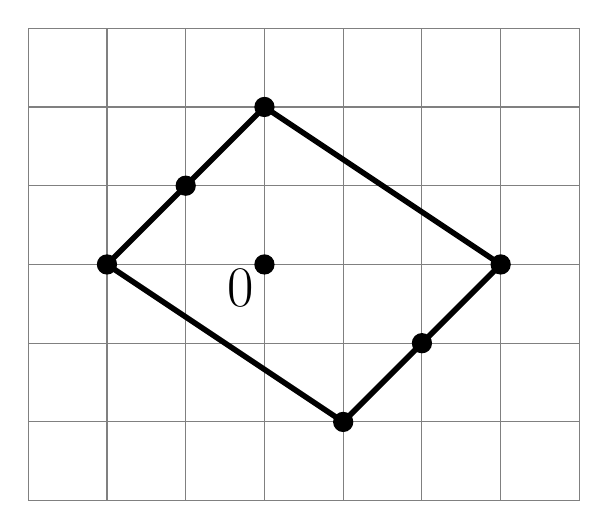
\begin{tikzpicture}
\draw [step=1,thin, gray] (-3,-3) grid (4,3);
\filldraw [ultra thick, fill=black] (0,0) circle [radius=0.1] ;
\node at (-0.3,-0.3){{\huge $0$}};

\filldraw [ultra thick, fill=black] (3,0) circle [radius=0.1] ; \filldraw [ultra thick, fill=black] (0,2) circle [radius=0.1] ;
\filldraw [ultra thick, fill=black] (-2,0) circle [radius=0.1] ; \filldraw [ultra thick, fill=black] (1,-2) circle [radius=0.1] ;
\filldraw [ultra thick, fill=black] (2,-1) circle [radius=0.1] ; \filldraw [ultra thick, fill=black] (-1,1) circle [radius=0.1] ;

\draw[line width=0.07cm] (3,0)--(0,2)--(-2,0)--(1,-2)--(3,0) ;
\end{tikzpicture} } }
%\end{center}
\caption{}\label{ex_FIA}
\end{minipage}

\begin{minipage}{0.38\hsize}\centering
%\begin{center}
{\scalebox{0.5}{
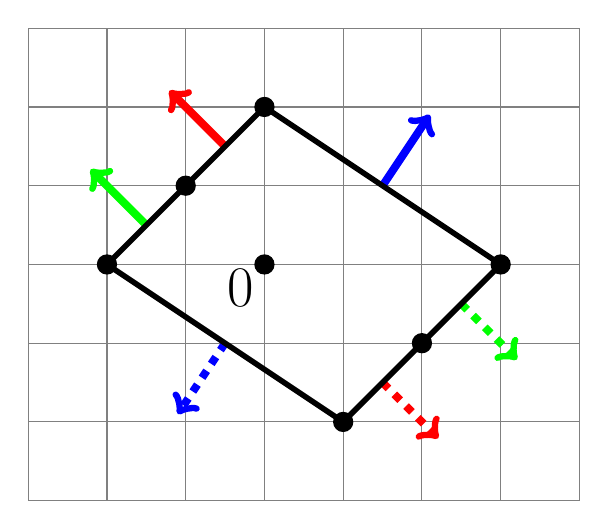
\begin{tikzpicture}
\draw [step=1,thin, gray] (-3,-3) grid (4,3);
\filldraw [ultra thick, fill=black] (0,0) circle [radius=0.1] ;
\node at (-0.3,-0.3){{\huge $0$}};

\filldraw [ultra thick, fill=black] (3,0) circle [radius=0.1] ; \filldraw [ultra thick, fill=black] (0,2) circle [radius=0.1] ;
\filldraw [ultra thick, fill=black] (-2,0) circle [radius=0.1] ; \filldraw [ultra thick, fill=black] (1,-2) circle [radius=0.1] ;
\filldraw [ultra thick, fill=black] (2,-1) circle [radius=0.1] ; \filldraw [ultra thick, fill=black] (-1,1) circle [radius=0.1] ;

\draw[->, dashed, line width=0.1cm,color=green] (2.5,-0.5)--++(-45:1);
\draw[->, dashed, line width=0.1cm,color=red] (1.5,-1.5)--++(-45:1);
\draw[->, line width=0.1cm,color=red] (-0.5,1.5)--++(135:1);
\draw[->, line width=0.1cm,color=green] (-1.5,0.5)--++(135:1);
\draw[->, line width=0.1cm,color=blue] (1.5,1)--++(0.6,0.9);
\draw[->, dashed, line width=0.1cm,color=blue] (-0.5,-1)--++(-0.6,-0.9);
\draw[line width=0.07cm] (3,0)--(0,2)--(-2,0)--(1,-2)--(3,0) ;
\end{tikzpicture} } }
%\end{center}
\caption{}\label{ex_FIA_orthogonal}
\end{minipage}
\end{tabular}
\end{figure}



\begin{enonce*}[remark]{Hanany--Vegh algorithm for a parallelogram~\cite{HV}}\ 
 
\begin{enumerate}%[(a)]
\item Consider primitive vectors orthogonal to each primitive side segments of the given polygon (see Figure~\ref{ex_FIA_orthogonal}).
\item Consider curves on the two-torus $\sfT$ whose homology classes coincide with the above vectors, and write such curves on $\sfT$ according to the following rules:
\begin{enumerate}%[(b-1)]
\item They induce a cell decomposition of $\sfT$.
\item Each curve intersects with other curves transversely and has a finite number of intersections.
\item No three curves intersect in the same point.
\item Tracing along each curve, we see that its intersections with other curves occur with alternating orientations. (For example, it is crossed from right to left and then left to right.)
\end{enumerate}
We call a resulting figure an \emph{admissible position} (see Figure~\ref{ex_FIA_homology}).
\item After these processes, we have three kinds of quadrangles that are oriented clockwise, anti-clockwise and alternately:
\begin{center}
{\scalebox{0.9}{
\begin{tikzpicture}

\node (CC1) at (0,0) {\scalebox{1.2}{
\begin{tikzpicture}
\coordinate (P1) at (0.5,0); \coordinate (P2) at (1,0.5); \coordinate (P3) at (0.5,1); \coordinate (P4) at (0,0.5);

\draw[line width=0.03cm] (0,0)--(1,0)--(1,1)--(0,1)--(0,0);
\draw[->, line width=0.03cm] (0,0)--(P4); \draw[->, line width=0.03cm] (1,0)--(P1);
\draw[->, line width=0.03cm] (1,1)--(P2); \draw[->, line width=0.03cm] (0,1)--(P3);
\end{tikzpicture} }};

\node (CC2) at (2.5,0) {\scalebox{1.2}{
\begin{tikzpicture}
\draw[line width=0.03cm] (0,0)--(1,0)--(1,1)--(0,1)--(0,0);
\draw[->, line width=0.03cm] (0,0)--(P1); \draw[->, line width=0.03cm] (1,0)--(P2);
\draw[->, line width=0.03cm] (1,1)--(P3); \draw[->, line width=0.03cm] (0,1)--(P4);
\end{tikzpicture} }} ;

\node (CC3) at (5,0) {\scalebox{1.2}{
\begin{tikzpicture}
\draw[line width=0.03cm] (0,0)--(1,0)--(1,1)--(0,1)--(0,0);
\draw[->, line width=0.03cm] (1,0)--(P1); \draw[->, line width=0.03cm] (1,0)--(P2);
\draw[->, line width=0.03cm] (0,1)--(P3); \draw[->, line width=0.03cm] (0,1)--(P4);
\end{tikzpicture} }};
\end{tikzpicture} }}
\end{center}

\item Draw white (resp. black) nodes in quadrangles oriented clockwise (resp. anti-clockwise).
\item Connect white nodes to black ones facing each other across intersections of curves.
\item Then, we obtain a square dimer model shown in Figure~\ref{ex_FIA_dimer}. We can check that this is isoradial, thus consistent in particular.
\end{enumerate}

\begin{figure}[H]
\centering
\begin{tabular}{c}
\begin{minipage}{0.4\hsize}\centering
%\begin{center}
{\scalebox{0.3}{
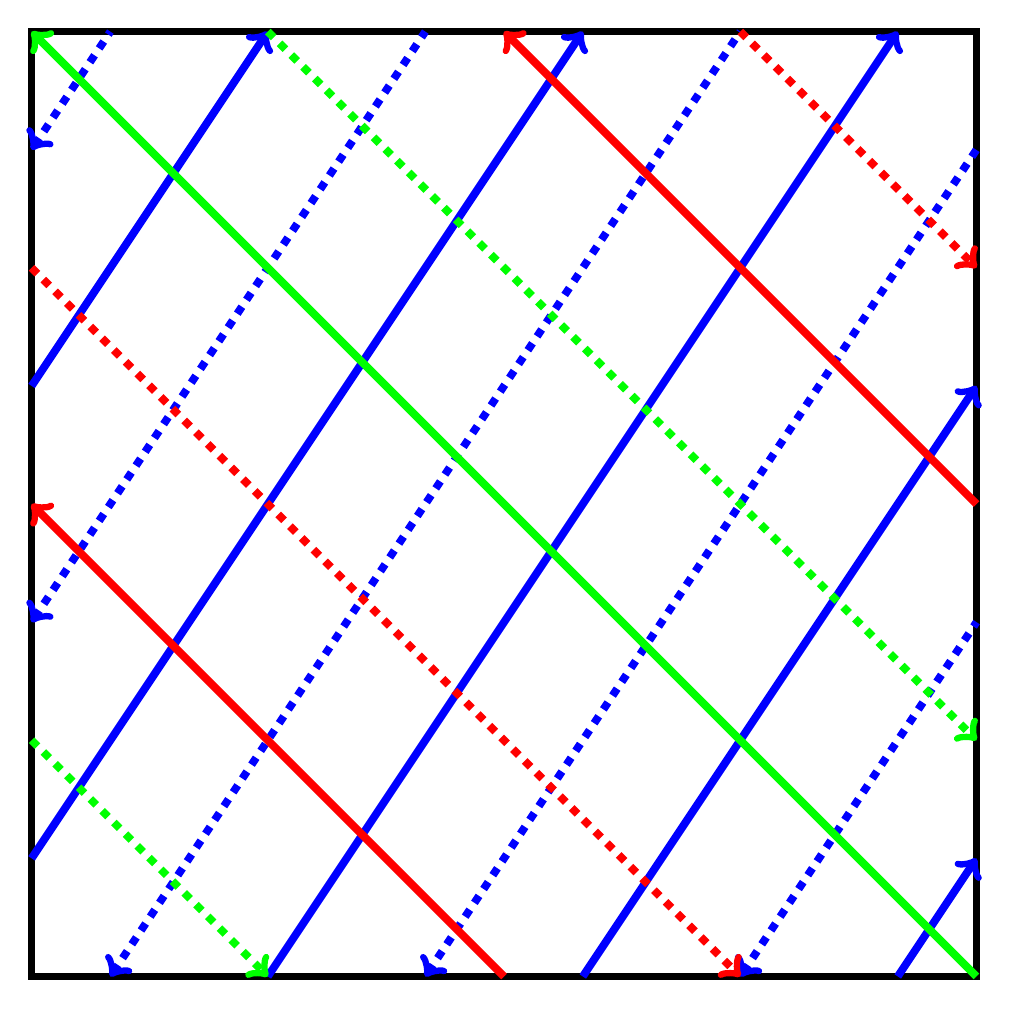
\begin{tikzpicture}
\draw[line width=0.08cm] (0,0) rectangle (12,12);

\draw[<-, dashed, line width=0.1cm,blue] (1,0)--(9,12);
\draw[<-, dashed, line width=0.1cm,blue] (5,0)--(12,10.5);
\draw[<-, dashed, line width=0.1cm,blue] (9,0)--(12,4.5);
\draw[<-, dashed, line width=0.1cm,blue] (0,4.5)--(5,12);
\draw[<-, dashed, line width=0.1cm,blue] (0,10.5)--(1,12);

\draw[->, line width=0.1cm, blue] (3,0)--(11,12);
\draw[->, line width=0.1cm, blue] (7,0)--(12,7.5);
\draw[->, line width=0.1cm, blue] (11,0)--(12,1.5);
\draw[->, line width=0.1cm, blue] (0,1.5)--(7,12);
\draw[->, line width=0.1cm, blue] (0,7.5)--(3,12);

\draw[->, line width=0.1cm,green] (12,0)--(0,12);
\draw[->, line width=0.1cm,red] (6,0)--(0,6); \draw[->, line width=0.1cm,red] (12,6)--(6,12);
\draw[->, dashed, line width=0.1cm,green] (0,3)--(3,0); \draw[->, dashed, line width=0.1cm,green] (3,12)--(12,3);
\draw[->, dashed, line width=0.1cm,red] (0,9)--(9,0); \draw[->, dashed, line width=0.1cm,red] (9,12)--(12,9);
\end{tikzpicture} } }
%\end{center}
\caption{}\label{ex_FIA_homology}
\end{minipage}

\begin{minipage}{0.4\hsize}\centering
%\begin{center}
{\scalebox{0.3}{
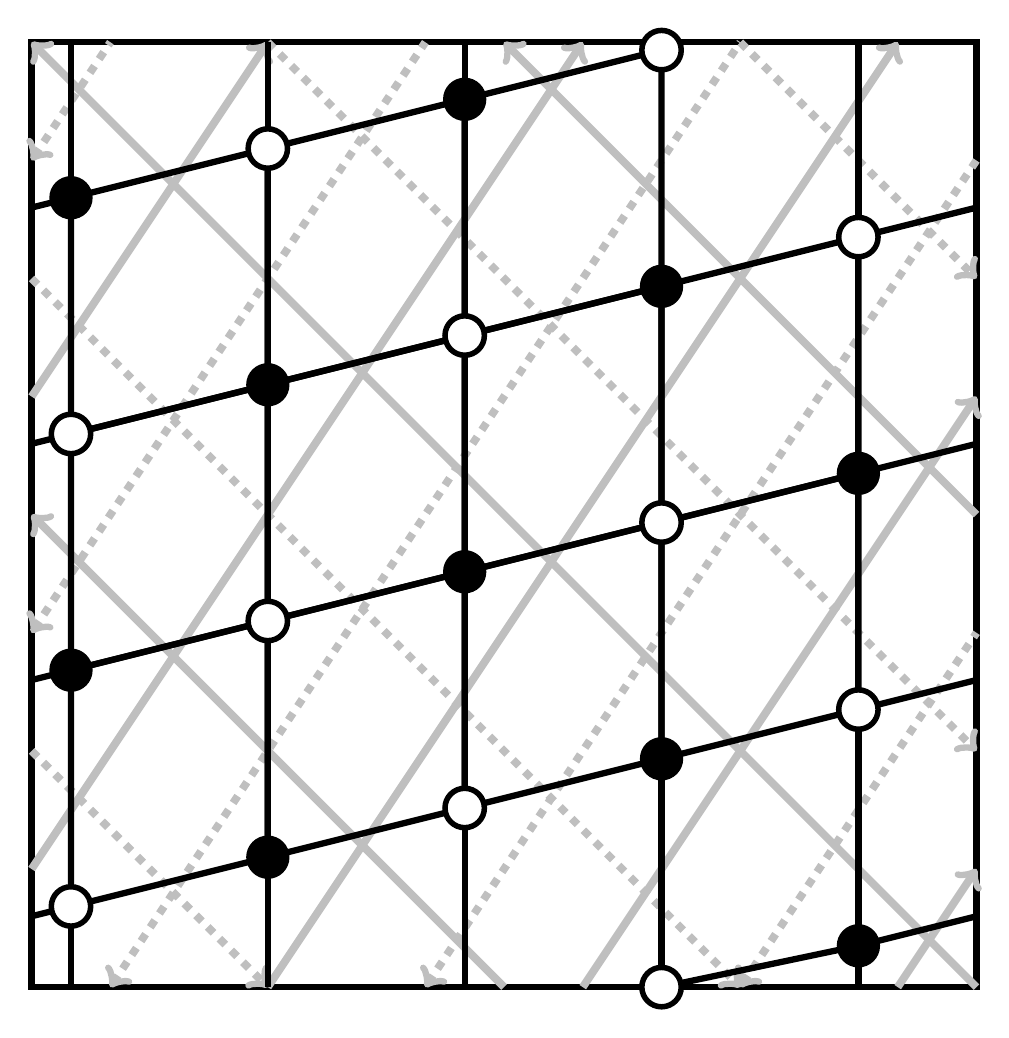
\begin{tikzpicture}
\draw[line width=0.08cm] (0,0) rectangle (12,12);

\draw[<-, dashed, line width=0.1cm,lightgray] (1,0)--(9,12);
\draw[<-, dashed, line width=0.1cm,lightgray] (5,0)--(12,10.5);
\draw[<-, dashed, line width=0.1cm,lightgray] (9,0)--(12,4.5);
\draw[<-, dashed, line width=0.1cm,lightgray] (0,4.5)--(5,12);
\draw[<-, dashed, line width=0.1cm,lightgray] (0,10.5)--(1,12);

\draw[->, line width=0.1cm,lightgray] (3,0)--(11,12);
\draw[->, line width=0.1cm,lightgray] (7,0)--(12,7.5);
\draw[->, line width=0.1cm,lightgray] (11,0)--(12,1.5);
\draw[->, line width=0.1cm,lightgray] (0,1.5)--(7,12);
\draw[->, line width=0.1cm,lightgray] (0,7.5)--(3,12);

\draw[->, line width=0.1cm,lightgray] (12,0)--(0,12);
\draw[->, line width=0.1cm,lightgray] (6,0)--(0,6); \draw[->, line width=0.1cm,lightgray] (12,6)--(6,12);
\draw[->, dashed, line width=0.1cm,lightgray] (0,3)--(3,0); \draw[->, dashed, line width=0.1cm,lightgray] (3,12)--(12,3);
\draw[->, dashed, line width=0.1cm,lightgray] (0,9)--(9,0); \draw[->, dashed, line width=0.1cm,lightgray] (9,12)--(12,9);

\coordinate (B1) at (0.5,4.025); \coordinate (B2) at (0.5,10.025); \coordinate (B3) at (3,1.65); \coordinate (B4) at (3,7.65);
\coordinate (B5) at (5.5,5.275); \coordinate (B6) at (5.5,11.275); \coordinate (B7) at (8,2.9); \coordinate (B8) at (8,8.9);
\coordinate (B9) at (10.5,0.525); \coordinate (B10) at (10.5,6.525);

\coordinate (W1) at (0.5,1.025); \coordinate (W2) at (0.5,7.025); \coordinate (W3) at (3,4.65); \coordinate (W4) at (3,10.65);
\coordinate (W5) at (5.5,2.275); \coordinate (W6) at (5.5,8.275); \coordinate (W7) at (8,5.9); \coordinate (W8) at (8,11.9); \coordinate (W8b) at (8,0);
\coordinate (W9) at (10.5,3.525); \coordinate (W10) at (10.5,9.525);


\draw[line width=0.08cm] (W1)--(B1)--(W3)--(B3)--(W1); \draw[line width=0.08cm] (W3)--(B3)--(W5)--(B5)--(W3);
\draw[line width=0.08cm] (W5)--(B5)--(W7)--(B7)--(W5); \draw[line width=0.08cm] (W7)--(B7)--(W9)--(B10)--(W7);
\draw[line width=0.08cm] (B1)--(W2)--(B4)--(W3)--(B1); \draw[line width=0.08cm] (B4)--(W6)--(B5)--(W3)--(B4);
\draw[line width=0.08cm] (B5)--(W6)--(B8)--(W7)--(B5); \draw[line width=0.08cm] (B8)--(W10)--(B10)--(W7)--(B8);
\draw[line width=0.08cm] (W2)--(B2)--(W4)--(B4)--(W2); \draw[line width=0.08cm] (W4)--(B4)--(W6)--(B6)--(W4);
\draw[line width=0.08cm] (W6)--(B6)--(W8)--(B8)--(W6); \draw[line width=0.08cm] (W8b)--(B9) ;

\draw[line width=0.08cm] (W1)--(0.5,0); \draw[line width=0.08cm] (B3)--(3,0); \draw[line width=0.08cm] (W5)--(5.5,0);
\draw[line width=0.08cm] (B7)--(8,0); \draw[line width=0.08cm] (W9)--(10.5,0);
\draw[line width=0.08cm] (B2)--(0.5,12); \draw[line width=0.08cm] (W4)--(3,12); \draw[line width=0.08cm] (B6)--(5.5,12);
\draw[line width=0.08cm] (W8)--(8,12); \draw[line width=0.08cm] (W10)--(10.5,12);

\draw[line width=0.08cm] (W1)--(0,0.9); \draw[line width=0.08cm] (B1)--(0,3.9); \draw[line width=0.08cm] (W2)--(0,6.9);
\draw[line width=0.08cm] (B2)--(0,9.9); \draw[line width=0.08cm] (W9)--(12,3.9); \draw[line width=0.08cm] (B10)--(12,6.9);
\draw[line width=0.08cm] (W10)--(12,9.9); \draw[line width=0.08cm] (B9)--(12,0.9);

\filldraw [line width=0.05cm, fill=black] (B1) circle [radius=0.25] ; \filldraw [line width=0.05cm, fill=black] (B2) circle [radius=0.25] ;
\filldraw [line width=0.05cm, fill=black] (B3) circle [radius=0.25] ; \filldraw [line width=0.05cm, fill=black] (B4) circle [radius=0.25] ;
\filldraw [line width=0.05cm, fill=black] (B5) circle [radius=0.25] ; \filldraw [line width=0.05cm, fill=black] (B6) circle [radius=0.25] ;
\filldraw [line width=0.05cm, fill=black] (B7) circle [radius=0.25] ; \filldraw [line width=0.05cm, fill=black] (B8) circle [radius=0.25] ;
\filldraw [line width=0.05cm, fill=black] (B9) circle [radius=0.25] ;
\filldraw [line width=0.05cm, fill=black] (B10) circle [radius=0.25] ;

\filldraw [line width=0.07cm, fill=white] (W1) circle [radius=0.25] ; \filldraw [line width=0.07cm, fill=white] (W2) circle [radius=0.25] ;
\filldraw [line width=0.07cm, fill=white] (W3) circle [radius=0.25] ; \filldraw [line width=0.07cm, fill=white] (W4) circle [radius=0.25] ;
\filldraw [line width=0.07cm, fill=white] (W5) circle [radius=0.25] ; \filldraw [line width=0.07cm, fill=white] (W6) circle [radius=0.25] ;
\filldraw [line width=0.07cm, fill=white] (W7) circle [radius=0.25] ; \filldraw [line width=0.07cm, fill=white] (W8) circle [radius=0.25] ;
\filldraw [line width=0.07cm, fill=white] (W8b) circle [radius=0.25] ;
\filldraw [line width=0.07cm, fill=white] (W9) circle [radius=0.25] ; \filldraw [line width=0.07cm, fill=white] (W10) circle [radius=0.25] ;
\end{tikzpicture} } }
%\end{center}
\caption{}\label{ex_FIA_dimer}
\end{minipage}
\end{tabular}
\end{figure}

Note that curves in an admissible position correspond to zigzag paths of the resulting consistent dimer model with the opposite direction. Thus, the correspondence in Proposition~\ref{zigzag_sidepolygon} asserts that the given parallelogram coincides with the perfect matching polygon by rotating $90$ degrees in the positive direction. Thus, we have the same lattice polygon up to unimodular transformations.

Using the same argument, we can obtain a dimer model that is homotopy equivalent to a square dimer model for an arbitrary parallelogram.

%\medskip

\end{enonce*}


Next, we show $\eqref{th4-2_2}\Rightarrow\eqref{th4-2_3}$.
Let $\Gamma$ be a dimer model associated with a given toric singularity $R$, and suppose that $\Gamma$ is homotopy equivalent to a square dimer model. Thus, the universal cover of $\Gamma$ takes the form shown in Figure~\ref{covering_square}, and Figure~\ref{zig_zag_square} is the list of zigzag paths on the universal cover. (They continue infinitely in both directions.) Since these zigzag paths determine four distinct slopes, the toric diagram of $R$ is a quadrangle by Proposition~\ref{zigzag_sidepolygon}. In addition, by observing these zigzag paths, we see that $\Gamma$ is isoradial.

\begin{figure}[htb]\centering
%\begin{center}
{\scalebox{0.35}{
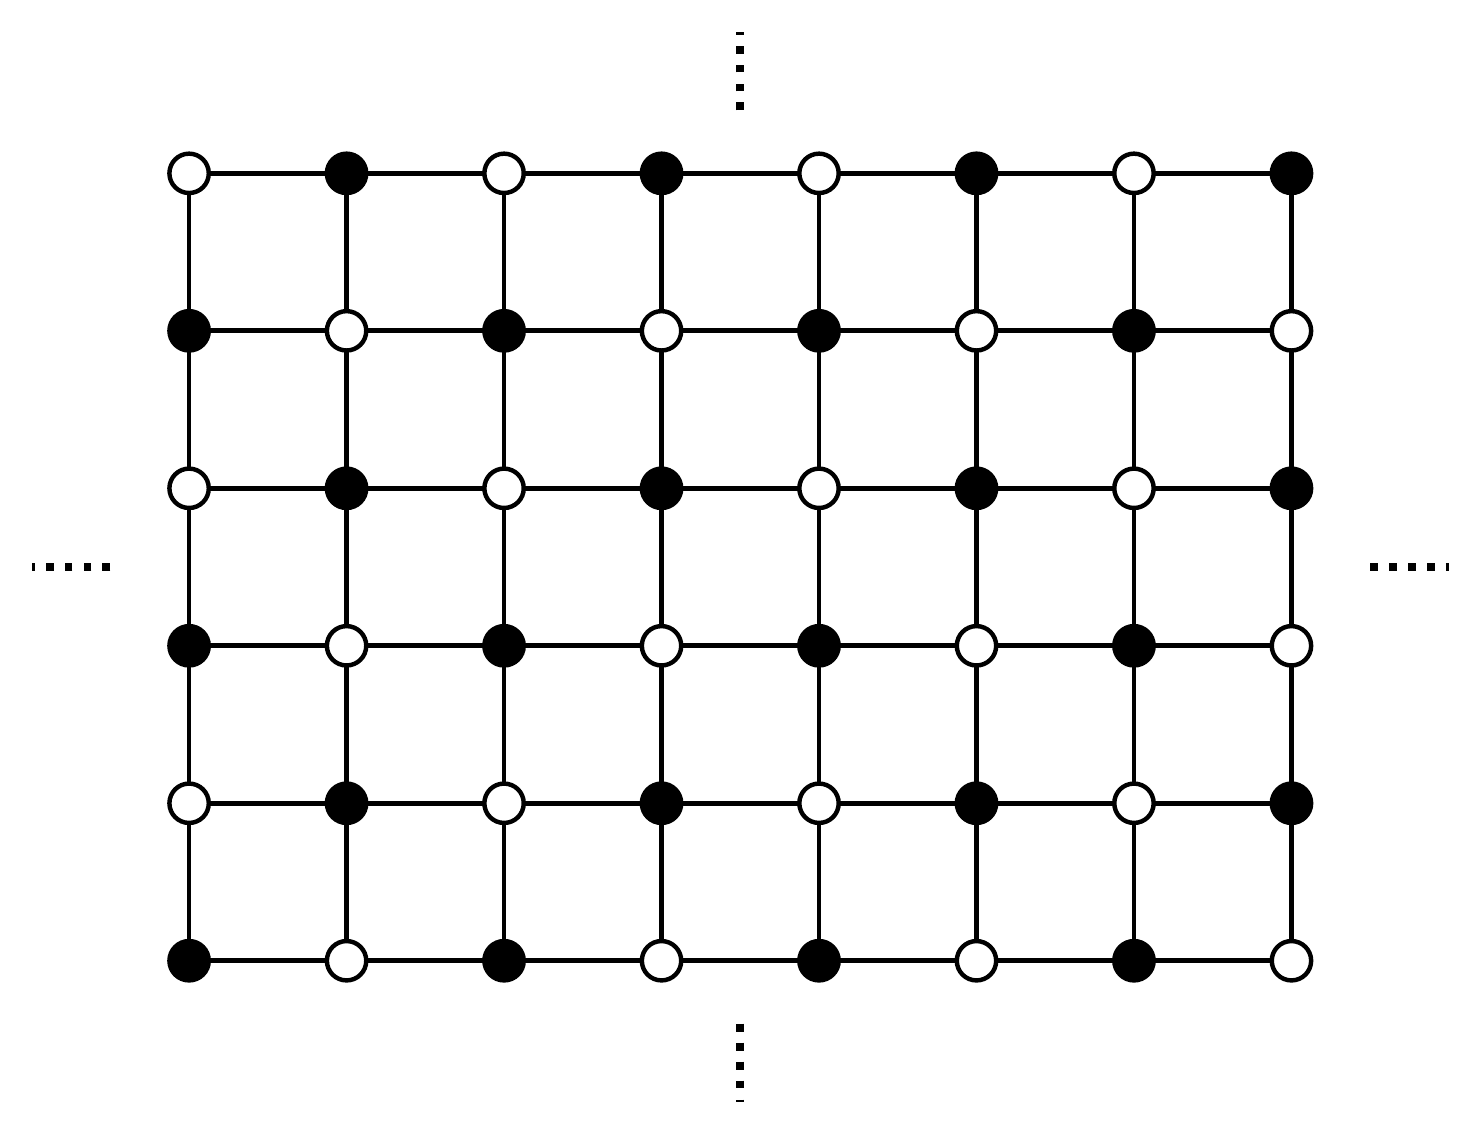
\begin{tikzpicture}
%vertex
\node (B1) at (0,0){$$}; \node (B2) at (4,0){$$}; \node (B3) at (8,0){$$}; \node (B4) at (12,0){$$}; 
\node (B5) at (2,2){$$}; \node (B6) at (6,2){$$}; \node (B7) at (10,2){$$}; \node (B8) at (14,2){$$}; 
\node (B9) at (0,4){$$}; \node (B10) at (4,4){$$}; \node (B11) at (8,4){$$}; \node (B12) at (12,4){$$}; 
\node (B13) at (2,6){$$}; \node (B14) at (6,6){$$}; \node (B15) at (10,6){$$}; \node (B16) at (14,6){$$};
\node (B17) at (0,8){$$}; \node (B18) at (4,8){$$}; \node (B19) at (8,8){$$}; \node (B20) at (12,8){$$}; 
\node (B21) at (2,10){$$}; \node (B22) at (6,10){$$}; \node (B23) at (10,10){$$}; \node (B24) at (14,10){$$};

\node (W1) at (2,0){$$}; \node (W2) at (6,0){$$}; \node (W3) at (10,0){$$}; \node (W4) at (14,0){$$}; 
\node (W5) at (0,2){$$}; \node (W6) at (4,2){$$}; \node (W7) at (8,2){$$}; \node (W8) at (12,2){$$};
\node (W9) at (2,4){$$}; \node (W10) at (6,4){$$}; \node (W11) at (10,4){$$}; \node (W12) at (14,4){$$}; 
\node (W13) at (0,6){$$}; \node (W14) at (4,6){$$}; \node (W15) at (8,6){$$}; \node (W16) at (12,6){$$};
\node (W17) at (2,8){$$}; \node (W18) at (6,8){$$}; \node (W19) at (10,8){$$}; \node (W20) at (14,8){$$}; 
\node (W21) at (0,10){$$}; \node (W22) at (4,10){$$}; \node (W23) at (8,10){$$}; \node (W24) at (12,10){$$};

%edge
\draw[line width=0.06cm] (B1)--(W1)--(B5)--(W5)--(B1); \draw[line width=0.06cm] (W1)--(B2)--(W6)--(B5)--(W1);
\draw[line width=0.06cm] (B2)--(W2)--(B6)--(W6)--(B2); \draw[line width=0.06cm] (W2)--(B3)--(W7)--(B6)--(W2);
\draw[line width=0.06cm] (B3)--(W3)--(B7)--(W7)--(B3); \draw[line width=0.06cm] (W3)--(B4)--(W8)--(B7)--(W3);
\draw[line width=0.06cm] (B4)--(W4)--(B8)--(W8)--(B4); 

\draw[line width=0.06cm] (W5)--(B5)--(W9)--(B9)--(W5); \draw[line width=0.06cm] (B5)--(W6)--(B10)--(W9)--(B5); 
\draw[line width=0.06cm] (W6)--(B6)--(W10)--(B10)--(W6); \draw[line width=0.06cm] (B6)--(W7)--(B11)--(W10)--(B6); 
\draw[line width=0.06cm] (W7)--(B7)--(W11)--(B11)--(W7); \draw[line width=0.06cm] (B7)--(W8)--(B12)--(W11)--(B7); 
\draw[line width=0.06cm] (W8)--(B8)--(W12)--(B12)--(W8); 

\draw[line width=0.06cm] (B9)--(W9)--(B13)--(W13)--(B9); \draw[line width=0.06cm] (W9)--(B10)--(W14)--(B13)--(W9);
\draw[line width=0.06cm] (B10)--(W10)--(B14)--(W14)--(B10); \draw[line width=0.06cm] (W10)--(B11)--(W15)--(B14)--(W10);
\draw[line width=0.06cm] (B11)--(W11)--(B15)--(W15)--(B11); \draw[line width=0.06cm] (W11)--(B12)--(W16)--(B15)--(W11);
\draw[line width=0.06cm] (B12)--(W12)--(B16)--(W16)--(B12); 

\draw[line width=0.06cm] (W13)--(B13)--(W17)--(B17)--(W13); \draw[line width=0.06cm] (B13)--(W14)--(B18)--(W17)--(B13); 
\draw[line width=0.06cm] (W14)--(B14)--(W18)--(B18)--(W14); \draw[line width=0.06cm] (B14)--(W15)--(B19)--(W18)--(B14); 
\draw[line width=0.06cm] (W15)--(B15)--(W19)--(B19)--(W15); \draw[line width=0.06cm] (B15)--(W16)--(B20)--(W19)--(B15); 
\draw[line width=0.06cm] (W16)--(B16)--(W20)--(B20)--(W16); 

\draw[line width=0.06cm] (B17)--(W17)--(B21)--(W21)--(B17); \draw[line width=0.06cm] (W17)--(B18)--(W22)--(B21)--(W17);
\draw[line width=0.06cm] (B18)--(W18)--(B22)--(W22)--(B18); \draw[line width=0.06cm] (W18)--(B19)--(W23)--(B22)--(W18);
\draw[line width=0.06cm] (B19)--(W19)--(B23)--(W23)--(B19); \draw[line width=0.06cm] (W19)--(B20)--(W24)--(B23)--(W19);
\draw[line width=0.06cm] (B20)--(W20)--(B24)--(W24)--(B20); 

%black
\filldraw [ultra thick, fill=black] (0,0) circle [radius=0.25] ; \filldraw [ultra thick, fill=black] (4,0) circle [radius=0.25] ;
\filldraw [ultra thick, fill=black] (8,0) circle [radius=0.25] ; \filldraw [ultra thick, fill=black] (12,0) circle [radius=0.25] ; 
\filldraw [ultra thick, fill=black] (2,2) circle [radius=0.25] ; \filldraw [ultra thick, fill=black] (6,2) circle [radius=0.25] ;
\filldraw [ultra thick, fill=black] (10,2) circle [radius=0.25] ; \filldraw [ultra thick, fill=black] (14,2) circle [radius=0.25] ;

\filldraw [ultra thick, fill=black] (0,4) circle [radius=0.25] ; \filldraw [ultra thick, fill=black] (4,4) circle [radius=0.25] ;
\filldraw [ultra thick, fill=black] (8,4) circle [radius=0.25] ; \filldraw [ultra thick, fill=black] (12,4) circle [radius=0.25] ;
\filldraw [ultra thick, fill=black] (2,6) circle [radius=0.25] ; \filldraw [ultra thick, fill=black] (6,6) circle [radius=0.25] ;
\filldraw [ultra thick, fill=black] (10,6) circle [radius=0.25] ; \filldraw [ultra thick, fill=black] (14,6) circle [radius=0.25] ;

\filldraw [ultra thick, fill=black] (0,8) circle [radius=0.25] ; \filldraw [ultra thick, fill=black] (4,8) circle [radius=0.25] ;
\filldraw [ultra thick, fill=black] (8,8) circle [radius=0.25] ; \filldraw [ultra thick, fill=black] (12,8) circle [radius=0.25] ;
\filldraw [ultra thick, fill=black] (2,10) circle [radius=0.25] ; \filldraw [ultra thick, fill=black] (6,10) circle [radius=0.25] ;
\filldraw [ultra thick, fill=black] (10,10) circle [radius=0.25] ; \filldraw [ultra thick, fill=black] (14,10) circle [radius=0.25] ;

%white
\filldraw [ultra thick, fill=white] (2,0) circle [radius=0.25] ; \filldraw [ultra thick, fill=white] (6,0) circle [radius=0.25] ;
\filldraw [ultra thick, fill=white] (10,0) circle [radius=0.25] ; \filldraw [ultra thick, fill=white] (14,0) circle [radius=0.25] ;
\filldraw [ultra thick, fill=white] (0,2) circle [radius=0.25] ; \filldraw [ultra thick, fill=white] (4,2) circle [radius=0.25] ;
\filldraw [ultra thick, fill=white] (8,2) circle [radius=0.25] ; \filldraw [ultra thick, fill=white] (12,2) circle [radius=0.25] ;

\filldraw [ultra thick, fill=white] (2,4) circle [radius=0.25] ; \filldraw [ultra thick, fill=white] (6,4) circle [radius=0.25] ;
\filldraw [ultra thick, fill=white] (10,4) circle [radius=0.25] ; \filldraw [ultra thick, fill=white] (14,4) circle [radius=0.25] ;
\filldraw [ultra thick, fill=white] (0,6) circle [radius=0.25] ; \filldraw [ultra thick, fill=white] (4,6) circle [radius=0.25] ;
\filldraw [ultra thick, fill=white] (8,6) circle [radius=0.25] ; \filldraw [ultra thick, fill=white] (12,6) circle [radius=0.25] ;

\filldraw [ultra thick, fill=white] (2,8) circle [radius=0.25] ; \filldraw [ultra thick, fill=white] (6,8) circle [radius=0.25] ;
\filldraw [ultra thick, fill=white] (10,8) circle [radius=0.25] ; \filldraw [ultra thick, fill=white] (14,8) circle [radius=0.25] ;
\filldraw [ultra thick, fill=white] (0,10) circle [radius=0.25] ; \filldraw [ultra thick, fill=white] (4,10) circle [radius=0.25] ;
\filldraw [ultra thick, fill=white] (8,10) circle [radius=0.25] ; \filldraw [ultra thick, fill=white] (12,10) circle [radius=0.25] ;

\draw[loosely dotted, line width=0.1cm] (7,-0.8)--(7,-1.8) ; \draw[loosely dotted, line width=0.1cm] (7,10.8)--(7,11.8) ;
\draw[loosely dotted, line width=0.1cm] (-1,5)--(-2,5) ; \draw[loosely dotted, line width=0.1cm] (15,5)--(16,5) ;
\end{tikzpicture}
} }
\caption{The universal cover of a square dimer model}
\label{covering_square}
%\end{center}
\end{figure}

\begin{figure}[htb]
\centering
{\scalebox{0.95}{
\begin{tikzpicture}
\node (ZZ1) at (0,0) {\scalebox{0.3}{
\begin{tikzpicture}
\coordinate (B1) at (0,0); \coordinate (B2) at (4,0); \coordinate (B3) at (8,0); \coordinate (B4) at (12,0);
\coordinate (B5) at (2,2); \coordinate (B6) at (6,2); \coordinate (B7) at (10,2); \coordinate (B8) at (14,2);
\coordinate (B9) at (0,4); \coordinate (B10) at (4,4); \coordinate (B11) at (8,4); \coordinate (B12) at (12,4);
\coordinate (B13) at (2,6); \coordinate (B14) at (6,6); \coordinate (B15) at (10,6); \coordinate (B16) at (14,6);
\coordinate (B17) at (0,8); \coordinate (B18) at (4,8); \coordinate (B19) at (8,8); \coordinate (B20) at (12,8);
\coordinate (B21) at (2,10); \coordinate (B22) at (6,10); \coordinate (B23) at (10,10); \coordinate (B24) at (14,10);

\coordinate (W1) at (2,0); \coordinate (W2) at (6,0); \coordinate (W3) at (10,0); \coordinate (W4) at (14,0);
\coordinate (W5) at (0,2); \coordinate (W6) at (4,2); \coordinate (W7) at (8,2); \coordinate (W8) at (12,2);
\coordinate (W9) at (2,4); \coordinate (W10) at (6,4); \coordinate (W11) at (10,4); \coordinate (W12) at (14,4);
\coordinate (W13) at (0,6); \coordinate (W14) at (4,6); \coordinate (W15) at (8,6); \coordinate (W16) at (12,6);
\coordinate (W17) at (2,8); \coordinate (W18) at (6,8); \coordinate (W19) at (10,8); \coordinate (W20) at (14,8);
\coordinate (W21) at (0,10); \coordinate (W22) at (4,10); \coordinate (W23) at (8,10); \coordinate (W24) at (12,10);

\draw[line width=0.06cm] (B1)--(W1)--(B5)--(W5)--(B1); \draw[line width=0.06cm] (W1)--(B2)--(W6)--(B5)--(W1);
\draw[line width=0.06cm] (B2)--(W2)--(B6)--(W6)--(B2); \draw[line width=0.06cm] (W2)--(B3)--(W7)--(B6)--(W2);
\draw[line width=0.06cm] (B3)--(W3)--(B7)--(W7)--(B3); \draw[line width=0.06cm] (W3)--(B4)--(W8)--(B7)--(W3);
\draw[line width=0.06cm] (B4)--(W4)--(B8)--(W8)--(B4);

\draw[line width=0.06cm] (W5)--(B5)--(W9)--(B9)--(W5); \draw[line width=0.06cm] (B5)--(W6)--(B10)--(W9)--(B5);
\draw[line width=0.06cm] (W6)--(B6)--(W10)--(B10)--(W6); \draw[line width=0.06cm] (B6)--(W7)--(B11)--(W10)--(B6);
\draw[line width=0.06cm] (W7)--(B7)--(W11)--(B11)--(W7); \draw[line width=0.06cm] (B7)--(W8)--(B12)--(W11)--(B7);
\draw[line width=0.06cm] (W8)--(B8)--(W12)--(B12)--(W8);

\draw[line width=0.06cm] (B9)--(W9)--(B13)--(W13)--(B9); \draw[line width=0.06cm] (W9)--(B10)--(W14)--(B13)--(W9);
\draw[line width=0.06cm] (B10)--(W10)--(B14)--(W14)--(B10); \draw[line width=0.06cm] (W10)--(B11)--(W15)--(B14)--(W10);
\draw[line width=0.06cm] (B11)--(W11)--(B15)--(W15)--(B11); \draw[line width=0.06cm] (W11)--(B12)--(W16)--(B15)--(W11);
\draw[line width=0.06cm] (B12)--(W12)--(B16)--(W16)--(B12);

\draw[line width=0.06cm] (W13)--(B13)--(W17)--(B17)--(W13); \draw[line width=0.06cm] (B13)--(W14)--(B18)--(W17)--(B13);
\draw[line width=0.06cm] (W14)--(B14)--(W18)--(B18)--(W14); \draw[line width=0.06cm] (B14)--(W15)--(B19)--(W18)--(B14);
\draw[line width=0.06cm] (W15)--(B15)--(W19)--(B19)--(W15); \draw[line width=0.06cm] (B15)--(W16)--(B20)--(W19)--(B15);
\draw[line width=0.06cm] (W16)--(B16)--(W20)--(B20)--(W16);

\draw[line width=0.06cm] (B17)--(W17)--(B21)--(W21)--(B17); \draw[line width=0.06cm] (W17)--(B18)--(W22)--(B21)--(W17);
\draw[line width=0.06cm] (B18)--(W18)--(B22)--(W22)--(B18); \draw[line width=0.06cm] (W18)--(B19)--(W23)--(B22)--(W18);
\draw[line width=0.06cm] (B19)--(W19)--(B23)--(W23)--(B19); \draw[line width=0.06cm] (W19)--(B20)--(W24)--(B23)--(W19);
\draw[line width=0.06cm] (B20)--(W20)--(B24)--(W24)--(B20);

\filldraw [ultra thick, fill=black] (0,0) circle [radius=0.25] ; \filldraw [ultra thick, fill=black] (4,0) circle [radius=0.25] ;
\filldraw [ultra thick, fill=black] (8,0) circle [radius=0.25] ; \filldraw [ultra thick, fill=black] (12,0) circle [radius=0.25] ;
\filldraw [ultra thick, fill=black] (2,2) circle [radius=0.25] ; \filldraw [ultra thick, fill=black] (6,2) circle [radius=0.25] ;
\filldraw [ultra thick, fill=black] (10,2) circle [radius=0.25] ; \filldraw [ultra thick, fill=black] (14,2) circle [radius=0.25] ;

\filldraw [ultra thick, fill=black] (0,4) circle [radius=0.25] ; \filldraw [ultra thick, fill=black] (4,4) circle [radius=0.25] ;
\filldraw [ultra thick, fill=black] (8,4) circle [radius=0.25] ; \filldraw [ultra thick, fill=black] (12,4) circle [radius=0.25] ;
\filldraw [ultra thick, fill=black] (2,6) circle [radius=0.25] ; \filldraw [ultra thick, fill=black] (6,6) circle [radius=0.25] ;
\filldraw [ultra thick, fill=black] (10,6) circle [radius=0.25] ; \filldraw [ultra thick, fill=black] (14,6) circle [radius=0.25] ;

\filldraw [ultra thick, fill=black] (0,8) circle [radius=0.25] ; \filldraw [ultra thick, fill=black] (4,8) circle [radius=0.25] ;
\filldraw [ultra thick, fill=black] (8,8) circle [radius=0.25] ; \filldraw [ultra thick, fill=black] (12,8) circle [radius=0.25] ;
\filldraw [ultra thick, fill=black] (2,10) circle [radius=0.25] ; \filldraw [ultra thick, fill=black] (6,10) circle [radius=0.25] ;
\filldraw [ultra thick, fill=black] (10,10) circle [radius=0.25] ; \filldraw [ultra thick, fill=black] (14,10) circle [radius=0.25] ;

\filldraw [ultra thick, fill=white] (2,0) circle [radius=0.25] ; \filldraw [ultra thick, fill=white] (6,0) circle [radius=0.25] ;
\filldraw [ultra thick, fill=white] (10,0) circle [radius=0.25] ; \filldraw [ultra thick, fill=white] (14,0) circle [radius=0.25] ;
\filldraw [ultra thick, fill=white] (0,2) circle [radius=0.25] ; \filldraw [ultra thick, fill=white] (4,2) circle [radius=0.25] ;
\filldraw [ultra thick, fill=white] (8,2) circle [radius=0.25] ; \filldraw [ultra thick, fill=white] (12,2) circle [radius=0.25] ;

\filldraw [ultra thick, fill=white] (2,4) circle [radius=0.25] ; \filldraw [ultra thick, fill=white] (6,4) circle [radius=0.25] ;
\filldraw [ultra thick, fill=white] (10,4) circle [radius=0.25] ; \filldraw [ultra thick, fill=white] (14,4) circle [radius=0.25] ;
\filldraw [ultra thick, fill=white] (0,6) circle [radius=0.25] ; \filldraw [ultra thick, fill=white] (4,6) circle [radius=0.25] ;
\filldraw [ultra thick, fill=white] (8,6) circle [radius=0.25] ; \filldraw [ultra thick, fill=white] (12,6) circle [radius=0.25] ;

\filldraw [ultra thick, fill=white] (2,8) circle [radius=0.25] ; \filldraw [ultra thick, fill=white] (6,8) circle [radius=0.25] ;
\filldraw [ultra thick, fill=white] (10,8) circle [radius=0.25] ; \filldraw [ultra thick, fill=white] (14,8) circle [radius=0.25] ;
\filldraw [ultra thick, fill=white] (0,10) circle [radius=0.25] ; \filldraw [ultra thick, fill=white] (4,10) circle [radius=0.25] ;
\filldraw [ultra thick, fill=white] (8,10) circle [radius=0.25] ; \filldraw [ultra thick, fill=white] (12,10) circle [radius=0.25] ;

\draw[->, line width=0.25cm, rounded corners, color=red] (W1)--(B2)--(W6)--(B6)--(W10)--(B11)--(W15)--(B15)--(W19)--(B20)--(W24)--(B24) ;
\draw[->, line width=0.25cm, rounded corners, color=red] (B1)--(W5)--(B5)--(W9)--(B10)--(W14)--(B14)--(W18)--(B19)--(W23)--(B23);
\draw[->, line width=0.25cm, rounded corners, color=red] (B9)--(W13)--(B13)--(W17)--(B18)--(W22)--(B22) ;
\draw[->, line width=0.25cm, rounded corners, color=red] (B17)--(W21)--(B21) ;
\draw[->, line width=0.25cm, rounded corners, color=red] (W2)--(B3)--(W7)--(B7)--(W11)--(B12)--(W16)--(B16)--(W20) ;
\draw[->, line width=0.25cm, rounded corners, color=red] (W3)--(B4)--(W8)--(B8)--(W12) ;
\end{tikzpicture} } };

\node (ZZ2) at (6,0) {\scalebox{0.3}{
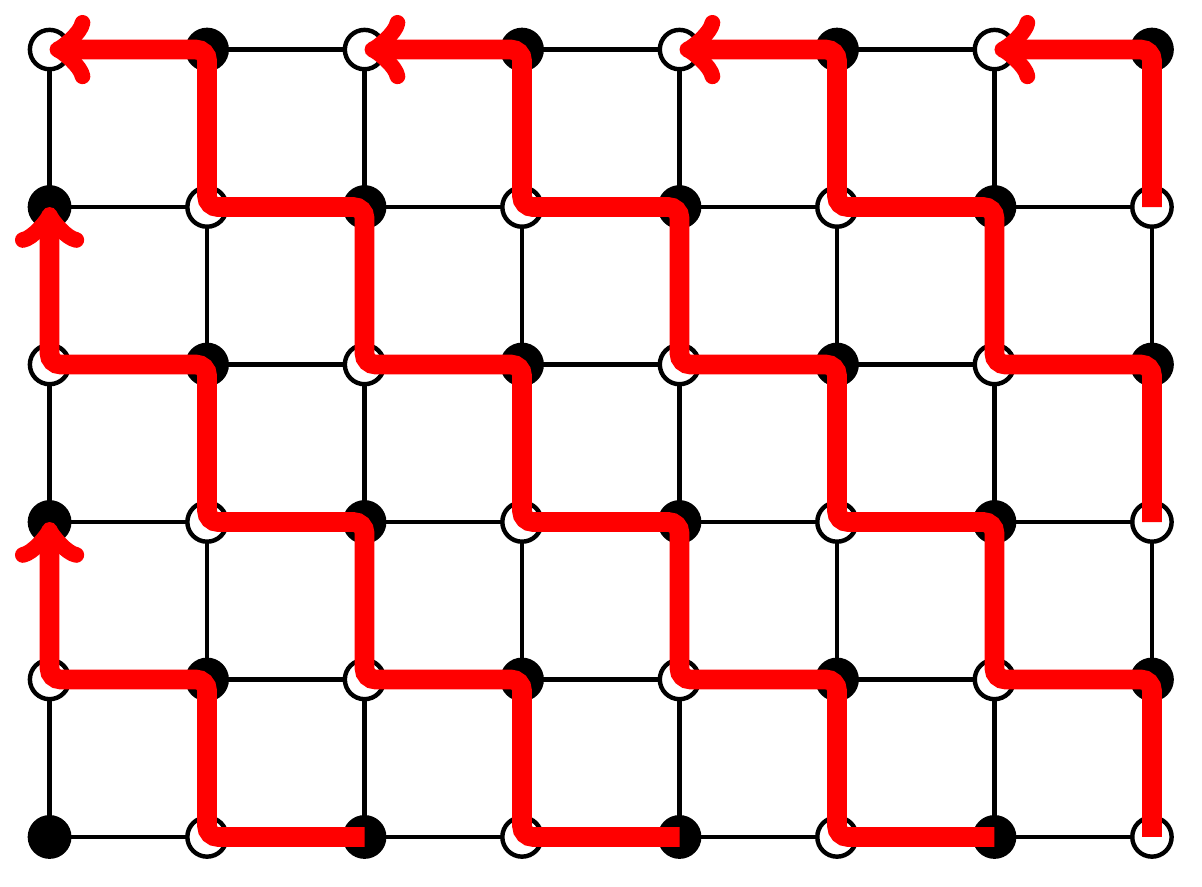
\begin{tikzpicture}
\coordinate (B1) at (0,0); \coordinate (B2) at (4,0); \coordinate (B3) at (8,0); \coordinate (B4) at (12,0);
\coordinate (B5) at (2,2); \coordinate (B6) at (6,2); \coordinate (B7) at (10,2); \coordinate (B8) at (14,2);
\coordinate (B9) at (0,4); \coordinate (B10) at (4,4); \coordinate (B11) at (8,4); \coordinate (B12) at (12,4);
\coordinate (B13) at (2,6); \coordinate (B14) at (6,6); \coordinate (B15) at (10,6); \coordinate (B16) at (14,6);
\coordinate (B17) at (0,8); \coordinate (B18) at (4,8); \coordinate (B19) at (8,8); \coordinate (B20) at (12,8);
\coordinate (B21) at (2,10); \coordinate (B22) at (6,10); \coordinate (B23) at (10,10); \coordinate (B24) at (14,10);

\coordinate (W1) at (2,0); \coordinate (W2) at (6,0); \coordinate (W3) at (10,0); \coordinate (W4) at (14,0);
\coordinate (W5) at (0,2); \coordinate (W6) at (4,2); \coordinate (W7) at (8,2); \coordinate (W8) at (12,2);
\coordinate (W9) at (2,4); \coordinate (W10) at (6,4); \coordinate (W11) at (10,4); \coordinate (W12) at (14,4);
\coordinate (W13) at (0,6); \coordinate (W14) at (4,6); \coordinate (W15) at (8,6); \coordinate (W16) at (12,6);
\coordinate (W17) at (2,8); \coordinate (W18) at (6,8); \coordinate (W19) at (10,8); \coordinate (W20) at (14,8);
\coordinate (W21) at (0,10); \coordinate (W22) at (4,10); \coordinate (W23) at (8,10); \coordinate (W24) at (12,10);

\draw[line width=0.06cm] (B1)--(W1)--(B5)--(W5)--(B1); \draw[line width=0.06cm] (W1)--(B2)--(W6)--(B5)--(W1);
\draw[line width=0.06cm] (B2)--(W2)--(B6)--(W6)--(B2); \draw[line width=0.06cm] (W2)--(B3)--(W7)--(B6)--(W2);
\draw[line width=0.06cm] (B3)--(W3)--(B7)--(W7)--(B3); \draw[line width=0.06cm] (W3)--(B4)--(W8)--(B7)--(W3);
\draw[line width=0.06cm] (B4)--(W4)--(B8)--(W8)--(B4);

\draw[line width=0.06cm] (W5)--(B5)--(W9)--(B9)--(W5); \draw[line width=0.06cm] (B5)--(W6)--(B10)--(W9)--(B5);
\draw[line width=0.06cm] (W6)--(B6)--(W10)--(B10)--(W6); \draw[line width=0.06cm] (B6)--(W7)--(B11)--(W10)--(B6);
\draw[line width=0.06cm] (W7)--(B7)--(W11)--(B11)--(W7); \draw[line width=0.06cm] (B7)--(W8)--(B12)--(W11)--(B7);
\draw[line width=0.06cm] (W8)--(B8)--(W12)--(B12)--(W8);

\draw[line width=0.06cm] (B9)--(W9)--(B13)--(W13)--(B9); \draw[line width=0.06cm] (W9)--(B10)--(W14)--(B13)--(W9);
\draw[line width=0.06cm] (B10)--(W10)--(B14)--(W14)--(B10); \draw[line width=0.06cm] (W10)--(B11)--(W15)--(B14)--(W10);
\draw[line width=0.06cm] (B11)--(W11)--(B15)--(W15)--(B11); \draw[line width=0.06cm] (W11)--(B12)--(W16)--(B15)--(W11);
\draw[line width=0.06cm] (B12)--(W12)--(B16)--(W16)--(B12);

\draw[line width=0.06cm] (W13)--(B13)--(W17)--(B17)--(W13); \draw[line width=0.06cm] (B13)--(W14)--(B18)--(W17)--(B13);
\draw[line width=0.06cm] (W14)--(B14)--(W18)--(B18)--(W14); \draw[line width=0.06cm] (B14)--(W15)--(B19)--(W18)--(B14);
\draw[line width=0.06cm] (W15)--(B15)--(W19)--(B19)--(W15); \draw[line width=0.06cm] (B15)--(W16)--(B20)--(W19)--(B15);
\draw[line width=0.06cm] (W16)--(B16)--(W20)--(B20)--(W16);

\draw[line width=0.06cm] (B17)--(W17)--(B21)--(W21)--(B17); \draw[line width=0.06cm] (W17)--(B18)--(W22)--(B21)--(W17);
\draw[line width=0.06cm] (B18)--(W18)--(B22)--(W22)--(B18); \draw[line width=0.06cm] (W18)--(B19)--(W23)--(B22)--(W18);
\draw[line width=0.06cm] (B19)--(W19)--(B23)--(W23)--(B19); \draw[line width=0.06cm] (W19)--(B20)--(W24)--(B23)--(W19);
\draw[line width=0.06cm] (B20)--(W20)--(B24)--(W24)--(B20);

\filldraw [ultra thick, fill=black] (0,0) circle [radius=0.25] ; \filldraw [ultra thick, fill=black] (4,0) circle [radius=0.25] ;
\filldraw [ultra thick, fill=black] (8,0) circle [radius=0.25] ; \filldraw [ultra thick, fill=black] (12,0) circle [radius=0.25] ;
\filldraw [ultra thick, fill=black] (2,2) circle [radius=0.25] ; \filldraw [ultra thick, fill=black] (6,2) circle [radius=0.25] ;
\filldraw [ultra thick, fill=black] (10,2) circle [radius=0.25] ; \filldraw [ultra thick, fill=black] (14,2) circle [radius=0.25] ;

\filldraw [ultra thick, fill=black] (0,4) circle [radius=0.25] ; \filldraw [ultra thick, fill=black] (4,4) circle [radius=0.25] ;
\filldraw [ultra thick, fill=black] (8,4) circle [radius=0.25] ; \filldraw [ultra thick, fill=black] (12,4) circle [radius=0.25] ;
\filldraw [ultra thick, fill=black] (2,6) circle [radius=0.25] ; \filldraw [ultra thick, fill=black] (6,6) circle [radius=0.25] ;
\filldraw [ultra thick, fill=black] (10,6) circle [radius=0.25] ; \filldraw [ultra thick, fill=black] (14,6) circle [radius=0.25] ;

\filldraw [ultra thick, fill=black] (0,8) circle [radius=0.25] ; \filldraw [ultra thick, fill=black] (4,8) circle [radius=0.25] ;
\filldraw [ultra thick, fill=black] (8,8) circle [radius=0.25] ; \filldraw [ultra thick, fill=black] (12,8) circle [radius=0.25] ;
\filldraw [ultra thick, fill=black] (2,10) circle [radius=0.25] ; \filldraw [ultra thick, fill=black] (6,10) circle [radius=0.25] ;
\filldraw [ultra thick, fill=black] (10,10) circle [radius=0.25] ; \filldraw [ultra thick, fill=black] (14,10) circle [radius=0.25] ;

\filldraw [ultra thick, fill=white] (2,0) circle [radius=0.25] ; \filldraw [ultra thick, fill=white] (6,0) circle [radius=0.25] ;
\filldraw [ultra thick, fill=white] (10,0) circle [radius=0.25] ; \filldraw [ultra thick, fill=white] (14,0) circle [radius=0.25] ;
\filldraw [ultra thick, fill=white] (0,2) circle [radius=0.25] ; \filldraw [ultra thick, fill=white] (4,2) circle [radius=0.25] ;
\filldraw [ultra thick, fill=white] (8,2) circle [radius=0.25] ; \filldraw [ultra thick, fill=white] (12,2) circle [radius=0.25] ;

\filldraw [ultra thick, fill=white] (2,4) circle [radius=0.25] ; \filldraw [ultra thick, fill=white] (6,4) circle [radius=0.25] ;
\filldraw [ultra thick, fill=white] (10,4) circle [radius=0.25] ; \filldraw [ultra thick, fill=white] (14,4) circle [radius=0.25] ;
\filldraw [ultra thick, fill=white] (0,6) circle [radius=0.25] ; \filldraw [ultra thick, fill=white] (4,6) circle [radius=0.25] ;
\filldraw [ultra thick, fill=white] (8,6) circle [radius=0.25] ; \filldraw [ultra thick, fill=white] (12,6) circle [radius=0.25] ;

\filldraw [ultra thick, fill=white] (2,8) circle [radius=0.25] ; \filldraw [ultra thick, fill=white] (6,8) circle [radius=0.25] ;
\filldraw [ultra thick, fill=white] (10,8) circle [radius=0.25] ; \filldraw [ultra thick, fill=white] (14,8) circle [radius=0.25] ;
\filldraw [ultra thick, fill=white] (0,10) circle [radius=0.25] ; \filldraw [ultra thick, fill=white] (4,10) circle [radius=0.25] ;
\filldraw [ultra thick, fill=white] (8,10) circle [radius=0.25] ; \filldraw [ultra thick, fill=white] (12,10) circle [radius=0.25] ;

\draw[->, line width=0.25cm, rounded corners, color=red] (W4)--(B8)--(W8)--(B12)--(W11)--(B15)--(W15)--(B19)--(W18)--(B22)--(W22) ;
\draw[->, line width=0.25cm, rounded corners, color=red] (B4)--(W3)--(B7)--(W7)--(B11)--(W10)--(B14)--(W14)--(B18)--(W17)--(B21)--(W21);
\draw[->, line width=0.25cm, rounded corners, color=red] (B3)--(W2)--(B6)--(W6)--(B10)--(W9)--(B13)--(W13)--(B17);
\draw[->, line width=0.25cm, rounded corners, color=red] (B2)--(W1)--(B5)--(W5)--(B9);
\draw[->, line width=0.25cm, rounded corners, color=red] (W12)--(B16)--(W16)--(B20)--(W19)--(B23)--(W23);
\draw[->, line width=0.25cm, rounded corners, color=red] (W20)--(B24)--(W24);
\end{tikzpicture} } };

\node (ZZ3) at (0,-4) {\scalebox{0.3}{
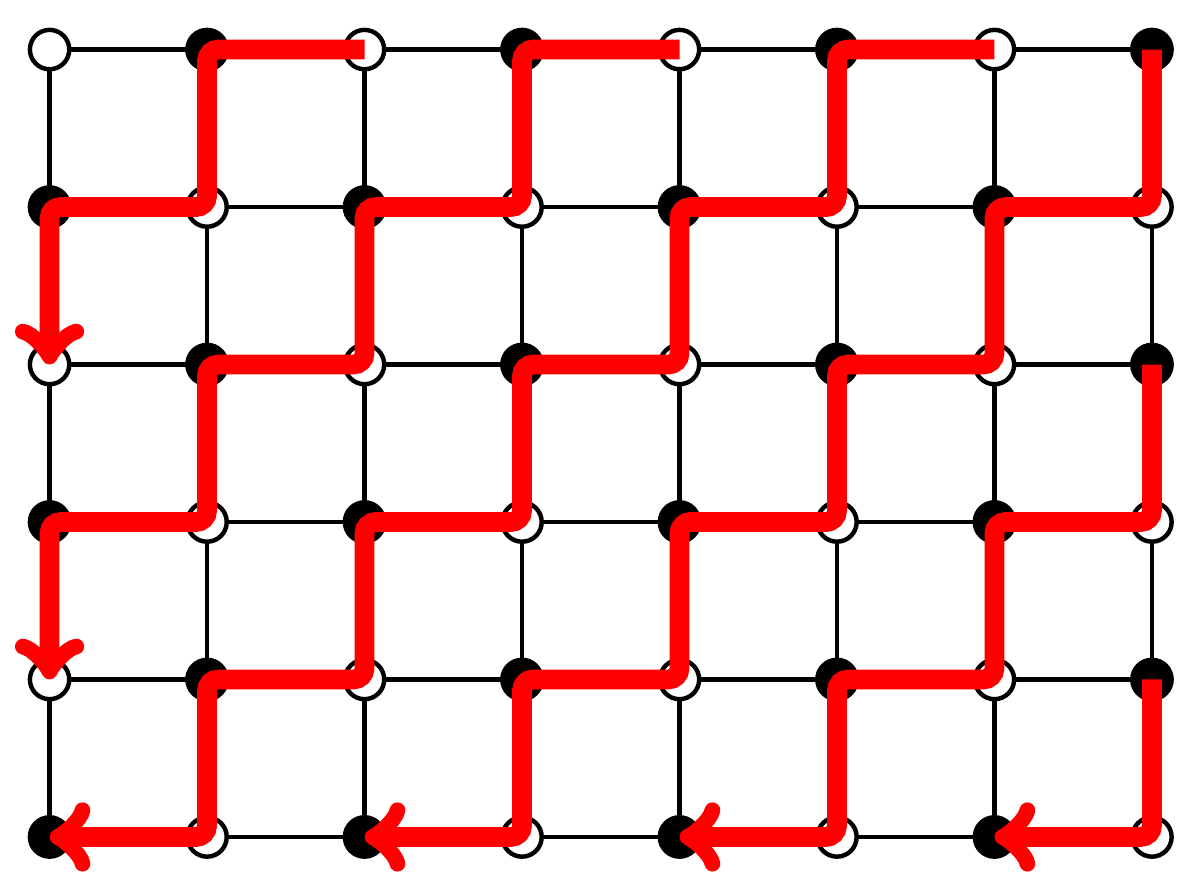
\begin{tikzpicture}
\coordinate (B1) at (0,0); \coordinate (B2) at (4,0); \coordinate (B3) at (8,0); \coordinate (B4) at (12,0);
\coordinate (B5) at (2,2); \coordinate (B6) at (6,2); \coordinate (B7) at (10,2); \coordinate (B8) at (14,2);
\coordinate (B9) at (0,4); \coordinate (B10) at (4,4); \coordinate (B11) at (8,4); \coordinate (B12) at (12,4);
\coordinate (B13) at (2,6); \coordinate (B14) at (6,6); \coordinate (B15) at (10,6); \coordinate (B16) at (14,6);
\coordinate (B17) at (0,8); \coordinate (B18) at (4,8); \coordinate (B19) at (8,8); \coordinate (B20) at (12,8);
\coordinate (B21) at (2,10); \coordinate (B22) at (6,10); \coordinate (B23) at (10,10); \coordinate (B24) at (14,10);

\coordinate (W1) at (2,0); \coordinate (W2) at (6,0); \coordinate (W3) at (10,0); \coordinate (W4) at (14,0);
\coordinate (W5) at (0,2); \coordinate (W6) at (4,2); \coordinate (W7) at (8,2); \coordinate (W8) at (12,2);
\coordinate (W9) at (2,4); \coordinate (W10) at (6,4); \coordinate (W11) at (10,4); \coordinate (W12) at (14,4);
\coordinate (W13) at (0,6); \coordinate (W14) at (4,6); \coordinate (W15) at (8,6); \coordinate (W16) at (12,6);
\coordinate (W17) at (2,8); \coordinate (W18) at (6,8); \coordinate (W19) at (10,8); \coordinate (W20) at (14,8);
\coordinate (W21) at (0,10); \coordinate (W22) at (4,10); \coordinate (W23) at (8,10); \coordinate (W24) at (12,10);

\draw[line width=0.06cm] (B1)--(W1)--(B5)--(W5)--(B1); \draw[line width=0.06cm] (W1)--(B2)--(W6)--(B5)--(W1);
\draw[line width=0.06cm] (B2)--(W2)--(B6)--(W6)--(B2); \draw[line width=0.06cm] (W2)--(B3)--(W7)--(B6)--(W2);
\draw[line width=0.06cm] (B3)--(W3)--(B7)--(W7)--(B3); \draw[line width=0.06cm] (W3)--(B4)--(W8)--(B7)--(W3);
\draw[line width=0.06cm] (B4)--(W4)--(B8)--(W8)--(B4);

\draw[line width=0.06cm] (W5)--(B5)--(W9)--(B9)--(W5); \draw[line width=0.06cm] (B5)--(W6)--(B10)--(W9)--(B5);
\draw[line width=0.06cm] (W6)--(B6)--(W10)--(B10)--(W6); \draw[line width=0.06cm] (B6)--(W7)--(B11)--(W10)--(B6);
\draw[line width=0.06cm] (W7)--(B7)--(W11)--(B11)--(W7); \draw[line width=0.06cm] (B7)--(W8)--(B12)--(W11)--(B7);
\draw[line width=0.06cm] (W8)--(B8)--(W12)--(B12)--(W8);

\draw[line width=0.06cm] (B9)--(W9)--(B13)--(W13)--(B9); \draw[line width=0.06cm] (W9)--(B10)--(W14)--(B13)--(W9);
\draw[line width=0.06cm] (B10)--(W10)--(B14)--(W14)--(B10); \draw[line width=0.06cm] (W10)--(B11)--(W15)--(B14)--(W10);
\draw[line width=0.06cm] (B11)--(W11)--(B15)--(W15)--(B11); \draw[line width=0.06cm] (W11)--(B12)--(W16)--(B15)--(W11);
\draw[line width=0.06cm] (B12)--(W12)--(B16)--(W16)--(B12);

\draw[line width=0.06cm] (W13)--(B13)--(W17)--(B17)--(W13); \draw[line width=0.06cm] (B13)--(W14)--(B18)--(W17)--(B13);
\draw[line width=0.06cm] (W14)--(B14)--(W18)--(B18)--(W14); \draw[line width=0.06cm] (B14)--(W15)--(B19)--(W18)--(B14);
\draw[line width=0.06cm] (W15)--(B15)--(W19)--(B19)--(W15); \draw[line width=0.06cm] (B15)--(W16)--(B20)--(W19)--(B15);
\draw[line width=0.06cm] (W16)--(B16)--(W20)--(B20)--(W16);

\draw[line width=0.06cm] (B17)--(W17)--(B21)--(W21)--(B17); \draw[line width=0.06cm] (W17)--(B18)--(W22)--(B21)--(W17);
\draw[line width=0.06cm] (B18)--(W18)--(B22)--(W22)--(B18); \draw[line width=0.06cm] (W18)--(B19)--(W23)--(B22)--(W18);
\draw[line width=0.06cm] (B19)--(W19)--(B23)--(W23)--(B19); \draw[line width=0.06cm] (W19)--(B20)--(W24)--(B23)--(W19);
\draw[line width=0.06cm] (B20)--(W20)--(B24)--(W24)--(B20);

\filldraw [ultra thick, fill=black] (0,0) circle [radius=0.25] ; \filldraw [ultra thick, fill=black] (4,0) circle [radius=0.25] ;
\filldraw [ultra thick, fill=black] (8,0) circle [radius=0.25] ; \filldraw [ultra thick, fill=black] (12,0) circle [radius=0.25] ;
\filldraw [ultra thick, fill=black] (2,2) circle [radius=0.25] ; \filldraw [ultra thick, fill=black] (6,2) circle [radius=0.25] ;
\filldraw [ultra thick, fill=black] (10,2) circle [radius=0.25] ; \filldraw [ultra thick, fill=black] (14,2) circle [radius=0.25] ;

\filldraw [ultra thick, fill=black] (0,4) circle [radius=0.25] ; \filldraw [ultra thick, fill=black] (4,4) circle [radius=0.25] ;
\filldraw [ultra thick, fill=black] (8,4) circle [radius=0.25] ; \filldraw [ultra thick, fill=black] (12,4) circle [radius=0.25] ;
\filldraw [ultra thick, fill=black] (2,6) circle [radius=0.25] ; \filldraw [ultra thick, fill=black] (6,6) circle [radius=0.25] ;
\filldraw [ultra thick, fill=black] (10,6) circle [radius=0.25] ; \filldraw [ultra thick, fill=black] (14,6) circle [radius=0.25] ;

\filldraw [ultra thick, fill=black] (0,8) circle [radius=0.25] ; \filldraw [ultra thick, fill=black] (4,8) circle [radius=0.25] ;
\filldraw [ultra thick, fill=black] (8,8) circle [radius=0.25] ; \filldraw [ultra thick, fill=black] (12,8) circle [radius=0.25] ;
\filldraw [ultra thick, fill=black] (2,10) circle [radius=0.25] ; \filldraw [ultra thick, fill=black] (6,10) circle [radius=0.25] ;
\filldraw [ultra thick, fill=black] (10,10) circle [radius=0.25] ; \filldraw [ultra thick, fill=black] (14,10) circle [radius=0.25] ;

\filldraw [ultra thick, fill=white] (2,0) circle [radius=0.25] ; \filldraw [ultra thick, fill=white] (6,0) circle [radius=0.25] ;
\filldraw [ultra thick, fill=white] (10,0) circle [radius=0.25] ; \filldraw [ultra thick, fill=white] (14,0) circle [radius=0.25] ;
\filldraw [ultra thick, fill=white] (0,2) circle [radius=0.25] ; \filldraw [ultra thick, fill=white] (4,2) circle [radius=0.25] ;
\filldraw [ultra thick, fill=white] (8,2) circle [radius=0.25] ; \filldraw [ultra thick, fill=white] (12,2) circle [radius=0.25] ;

\filldraw [ultra thick, fill=white] (2,4) circle [radius=0.25] ; \filldraw [ultra thick, fill=white] (6,4) circle [radius=0.25] ;
\filldraw [ultra thick, fill=white] (10,4) circle [radius=0.25] ; \filldraw [ultra thick, fill=white] (14,4) circle [radius=0.25] ;
\filldraw [ultra thick, fill=white] (0,6) circle [radius=0.25] ; \filldraw [ultra thick, fill=white] (4,6) circle [radius=0.25] ;
\filldraw [ultra thick, fill=white] (8,6) circle [radius=0.25] ; \filldraw [ultra thick, fill=white] (12,6) circle [radius=0.25] ;

\filldraw [ultra thick, fill=white] (2,8) circle [radius=0.25] ; \filldraw [ultra thick, fill=white] (6,8) circle [radius=0.25] ;
\filldraw [ultra thick, fill=white] (10,8) circle [radius=0.25] ; \filldraw [ultra thick, fill=white] (14,8) circle [radius=0.25] ;
\filldraw [ultra thick, fill=white] (0,10) circle [radius=0.25] ; \filldraw [ultra thick, fill=white] (4,10) circle [radius=0.25] ;
\filldraw [ultra thick, fill=white] (8,10) circle [radius=0.25] ; \filldraw [ultra thick, fill=white] (12,10) circle [radius=0.25] ;

\draw[->, line width=0.25cm, rounded corners, color=red] (W24)--(B23)--(W19)--(B19)--(W15)--(B14)--(W10)--(B10)--(W6)--(B5)--(W1)--(B1) ;
\draw[->, line width=0.25cm, rounded corners, color=red] (W23)--(B22)--(W18)--(B18)--(W14)--(B13)--(W9)--(B9)--(W5) ;
\draw[->, line width=0.25cm, rounded corners, color=red] (W22)--(B21)--(W17)--(B17)--(W13) ;
\draw[->, line width=0.25cm, rounded corners, color=red] (B24)--(W20)--(B20)--(W16)--(B15)--(W11)--(B11)--(W7)--(B6)--(W2)--(B2) ;
\draw[->, line width=0.25cm, rounded corners, color=red] (B16)--(W12)--(B12)--(W8)--(B7)--(W3)--(B3) ;
\draw[->, line width=0.25cm, rounded corners, color=red] (B8)--(W4)--(B4) ;
\end{tikzpicture} } };

\node (ZZ4) at (6,-4) {\scalebox{0.3}{
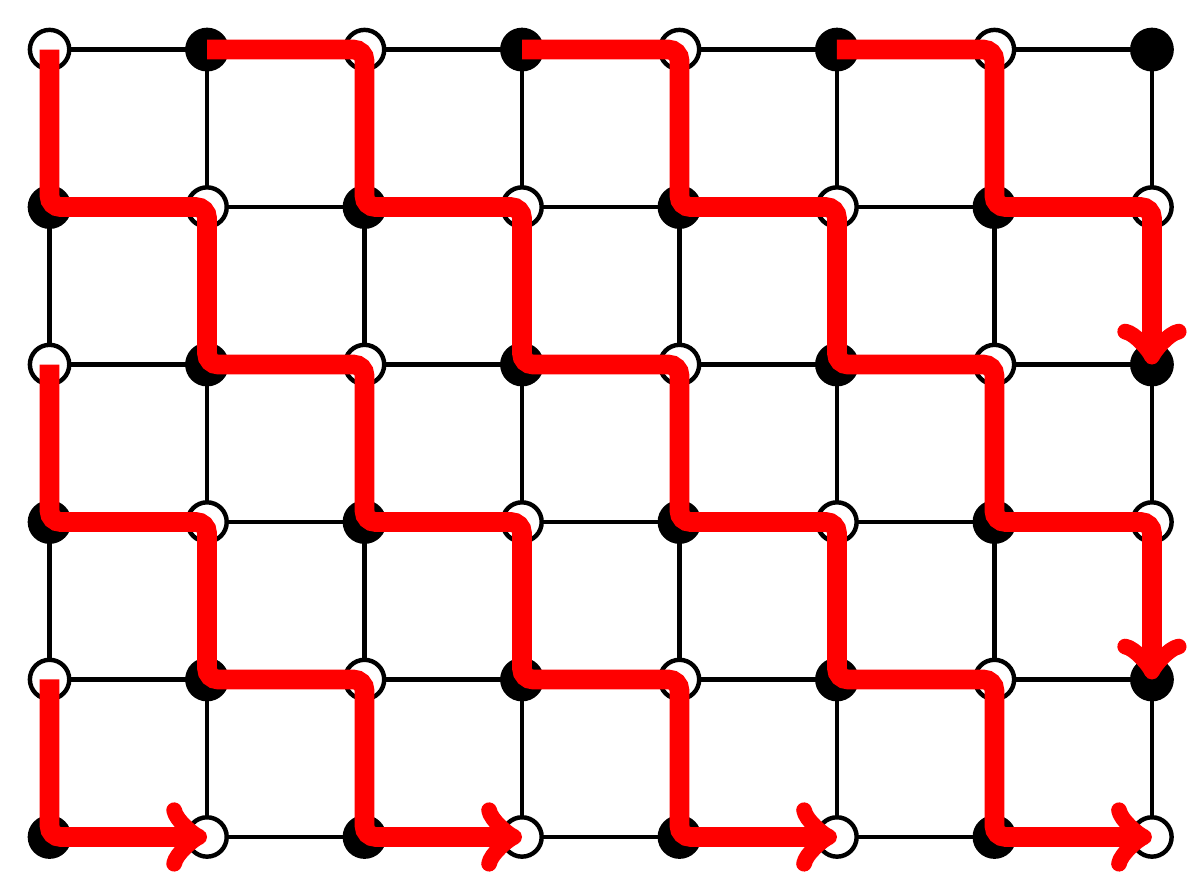
\begin{tikzpicture}
\coordinate (B1) at (0,0); \coordinate (B2) at (4,0); \coordinate (B3) at (8,0); \coordinate (B4) at (12,0);
\coordinate (B5) at (2,2); \coordinate (B6) at (6,2); \coordinate (B7) at (10,2); \coordinate (B8) at (14,2);
\coordinate (B9) at (0,4); \coordinate (B10) at (4,4); \coordinate (B11) at (8,4); \coordinate (B12) at (12,4);
\coordinate (B13) at (2,6); \coordinate (B14) at (6,6); \coordinate (B15) at (10,6); \coordinate (B16) at (14,6);
\coordinate (B17) at (0,8); \coordinate (B18) at (4,8); \coordinate (B19) at (8,8); \coordinate (B20) at (12,8);
\coordinate (B21) at (2,10); \coordinate (B22) at (6,10); \coordinate (B23) at (10,10); \coordinate (B24) at (14,10);

\coordinate (W1) at (2,0); \coordinate (W2) at (6,0); \coordinate (W3) at (10,0); \coordinate (W4) at (14,0);
\coordinate (W5) at (0,2); \coordinate (W6) at (4,2); \coordinate (W7) at (8,2); \coordinate (W8) at (12,2);
\coordinate (W9) at (2,4); \coordinate (W10) at (6,4); \coordinate (W11) at (10,4); \coordinate (W12) at (14,4);
\coordinate (W13) at (0,6); \coordinate (W14) at (4,6); \coordinate (W15) at (8,6); \coordinate (W16) at (12,6);
\coordinate (W17) at (2,8); \coordinate (W18) at (6,8); \coordinate (W19) at (10,8); \coordinate (W20) at (14,8);
\coordinate (W21) at (0,10); \coordinate (W22) at (4,10); \coordinate (W23) at (8,10); \coordinate (W24) at (12,10);

\draw[line width=0.06cm] (B1)--(W1)--(B5)--(W5)--(B1); \draw[line width=0.06cm] (W1)--(B2)--(W6)--(B5)--(W1);
\draw[line width=0.06cm] (B2)--(W2)--(B6)--(W6)--(B2); \draw[line width=0.06cm] (W2)--(B3)--(W7)--(B6)--(W2);
\draw[line width=0.06cm] (B3)--(W3)--(B7)--(W7)--(B3); \draw[line width=0.06cm] (W3)--(B4)--(W8)--(B7)--(W3);
\draw[line width=0.06cm] (B4)--(W4)--(B8)--(W8)--(B4);

\draw[line width=0.06cm] (W5)--(B5)--(W9)--(B9)--(W5); \draw[line width=0.06cm] (B5)--(W6)--(B10)--(W9)--(B5);
\draw[line width=0.06cm] (W6)--(B6)--(W10)--(B10)--(W6); \draw[line width=0.06cm] (B6)--(W7)--(B11)--(W10)--(B6);
\draw[line width=0.06cm] (W7)--(B7)--(W11)--(B11)--(W7); \draw[line width=0.06cm] (B7)--(W8)--(B12)--(W11)--(B7);
\draw[line width=0.06cm] (W8)--(B8)--(W12)--(B12)--(W8);

\draw[line width=0.06cm] (B9)--(W9)--(B13)--(W13)--(B9); \draw[line width=0.06cm] (W9)--(B10)--(W14)--(B13)--(W9);
\draw[line width=0.06cm] (B10)--(W10)--(B14)--(W14)--(B10); \draw[line width=0.06cm] (W10)--(B11)--(W15)--(B14)--(W10);
\draw[line width=0.06cm] (B11)--(W11)--(B15)--(W15)--(B11); \draw[line width=0.06cm] (W11)--(B12)--(W16)--(B15)--(W11);
\draw[line width=0.06cm] (B12)--(W12)--(B16)--(W16)--(B12);

\draw[line width=0.06cm] (W13)--(B13)--(W17)--(B17)--(W13); \draw[line width=0.06cm] (B13)--(W14)--(B18)--(W17)--(B13);
\draw[line width=0.06cm] (W14)--(B14)--(W18)--(B18)--(W14); \draw[line width=0.06cm] (B14)--(W15)--(B19)--(W18)--(B14);
\draw[line width=0.06cm] (W15)--(B15)--(W19)--(B19)--(W15); \draw[line width=0.06cm] (B15)--(W16)--(B20)--(W19)--(B15);
\draw[line width=0.06cm] (W16)--(B16)--(W20)--(B20)--(W16);

\draw[line width=0.06cm] (B17)--(W17)--(B21)--(W21)--(B17); \draw[line width=0.06cm] (W17)--(B18)--(W22)--(B21)--(W17);
\draw[line width=0.06cm] (B18)--(W18)--(B22)--(W22)--(B18); \draw[line width=0.06cm] (W18)--(B19)--(W23)--(B22)--(W18);
\draw[line width=0.06cm] (B19)--(W19)--(B23)--(W23)--(B19); \draw[line width=0.06cm] (W19)--(B20)--(W24)--(B23)--(W19);
\draw[line width=0.06cm] (B20)--(W20)--(B24)--(W24)--(B20);

\filldraw [ultra thick, fill=black] (0,0) circle [radius=0.25] ; \filldraw [ultra thick, fill=black] (4,0) circle [radius=0.25] ;
\filldraw [ultra thick, fill=black] (8,0) circle [radius=0.25] ; \filldraw [ultra thick, fill=black] (12,0) circle [radius=0.25] ;
\filldraw [ultra thick, fill=black] (2,2) circle [radius=0.25] ; \filldraw [ultra thick, fill=black] (6,2) circle [radius=0.25] ;
\filldraw [ultra thick, fill=black] (10,2) circle [radius=0.25] ; \filldraw [ultra thick, fill=black] (14,2) circle [radius=0.25] ;

\filldraw [ultra thick, fill=black] (0,4) circle [radius=0.25] ; \filldraw [ultra thick, fill=black] (4,4) circle [radius=0.25] ;
\filldraw [ultra thick, fill=black] (8,4) circle [radius=0.25] ; \filldraw [ultra thick, fill=black] (12,4) circle [radius=0.25] ;
\filldraw [ultra thick, fill=black] (2,6) circle [radius=0.25] ; \filldraw [ultra thick, fill=black] (6,6) circle [radius=0.25] ;
\filldraw [ultra thick, fill=black] (10,6) circle [radius=0.25] ; \filldraw [ultra thick, fill=black] (14,6) circle [radius=0.25] ;

\filldraw [ultra thick, fill=black] (0,8) circle [radius=0.25] ; \filldraw [ultra thick, fill=black] (4,8) circle [radius=0.25] ;
\filldraw [ultra thick, fill=black] (8,8) circle [radius=0.25] ; \filldraw [ultra thick, fill=black] (12,8) circle [radius=0.25] ;
\filldraw [ultra thick, fill=black] (2,10) circle [radius=0.25] ; \filldraw [ultra thick, fill=black] (6,10) circle [radius=0.25] ;
\filldraw [ultra thick, fill=black] (10,10) circle [radius=0.25] ; \filldraw [ultra thick, fill=black] (14,10) circle [radius=0.25] ;

\filldraw [ultra thick, fill=white] (2,0) circle [radius=0.25] ; \filldraw [ultra thick, fill=white] (6,0) circle [radius=0.25] ;
\filldraw [ultra thick, fill=white] (10,0) circle [radius=0.25] ; \filldraw [ultra thick, fill=white] (14,0) circle [radius=0.25] ;
\filldraw [ultra thick, fill=white] (0,2) circle [radius=0.25] ; \filldraw [ultra thick, fill=white] (4,2) circle [radius=0.25] ;
\filldraw [ultra thick, fill=white] (8,2) circle [radius=0.25] ; \filldraw [ultra thick, fill=white] (12,2) circle [radius=0.25] ;

\filldraw [ultra thick, fill=white] (2,4) circle [radius=0.25] ; \filldraw [ultra thick, fill=white] (6,4) circle [radius=0.25] ;
\filldraw [ultra thick, fill=white] (10,4) circle [radius=0.25] ; \filldraw [ultra thick, fill=white] (14,4) circle [radius=0.25] ;
\filldraw [ultra thick, fill=white] (0,6) circle [radius=0.25] ; \filldraw [ultra thick, fill=white] (4,6) circle [radius=0.25] ;
\filldraw [ultra thick, fill=white] (8,6) circle [radius=0.25] ; \filldraw [ultra thick, fill=white] (12,6) circle [radius=0.25] ;

\filldraw [ultra thick, fill=white] (2,8) circle [radius=0.25] ; \filldraw [ultra thick, fill=white] (6,8) circle [radius=0.25] ;
\filldraw [ultra thick, fill=white] (10,8) circle [radius=0.25] ; \filldraw [ultra thick, fill=white] (14,8) circle [radius=0.25] ;
\filldraw [ultra thick, fill=white] (0,10) circle [radius=0.25] ; \filldraw [ultra thick, fill=white] (4,10) circle [radius=0.25] ;
\filldraw [ultra thick, fill=white] (8,10) circle [radius=0.25] ; \filldraw [ultra thick, fill=white] (12,10) circle [radius=0.25] ;

\draw[->, line width=0.25cm, rounded corners, color=red] (B21)--(W22)--(B18)--(W18)--(B14)--(W15)--(B11)--(W11)--(B7)--(W8)--(B4)--(W4) ;
\draw[->, line width=0.25cm, rounded corners, color=red] (B22)--(W23)--(B19)--(W19)--(B15)--(W16)--(B12)--(W12)--(B8) ;
\draw[->, line width=0.25cm, rounded corners, color=red] (B23)--(W24)--(B20)--(W20)--(B16) ;
\draw[->, line width=0.25cm, rounded corners, color=red] (W21)--(B17)--(W17)--(B13)--(W14)--(B10)--(W10)--(B6)--(W7)--(B3)--(W3) ;
\draw[->, line width=0.25cm, rounded corners, color=red] (W13)--(B9)--(W9)--(B5)--(W6)--(B2)--(W2) ;
\draw[->, line width=0.25cm, rounded corners, color=red] (W5)--(B1)--(W1) ;
\end{tikzpicture} } };
\end{tikzpicture} }}
\caption{Zigzag paths on a square dimer model}\label{zig_zag_square}
\end{figure}

Let $(Q,W_Q)$ be the QP $(Q,W_Q)$ associated with $\Gamma$. By Theorem~\ref{NCCR1}, an MCM $R$-module
\[
e_i\calP(Q, W_Q)\cong\Hom_R\left(T_{ii}, \bigoplus_{j\in Q_0}T_{ij}\right)\cong\bigoplus_{j\in Q_0}T_{ij}
\]
gives an NCCR of $R$ for all $i\in Q_0$. Since we know that the toric diagram $\Delta$ of $R$ is a quadrangle, let $u_1,\dots,u_4\in\ZZ^2$ be vertices of $\Delta$, and we assume that these are ordered cyclically along $\Delta$. Since $\Gamma$ is consistent, there exists a unique extremal perfect matching, corresponding to each vertex. We denote extremal perfect matchings corresponding to $u_1,\dots,u_4$ by $\sfP_1,\dots, \sfP_4$ respectively. Here, we recall that each module $T_{ij}$ can be constructed from the perfect matching functions of extremal ones (see Subsection~\ref{sec_consist}). In our situation, extremal perfect matchings $\sfP_1,\dots,\sfP_4$ are of the form shown in Figure~\ref{expm_square}, because differences of adjacent extremal perfect matchings induce zigzag paths.

\begin{figure}[htb]\centering
{\scalebox{0.95}{
\begin{tikzpicture}
\node at (0,-2) {$\sfP_1$};\node at (6,-2) {$\sfP_2$}; 
\node at (0,-6.2) {$\sfP_3$}; \node at (6,-6.2) {$\sfP_4$}; 

\node (PM1) at (0,0) 
{\scalebox{0.3}{
\begin{tikzpicture}
%vertex
\node (B1) at (0,0){$$}; \node (B2) at (4,0){$$}; \node (B3) at (8,0){$$}; \node (B4) at (12,0){$$}; 
\node (B5) at (2,2){$$}; \node (B6) at (6,2){$$}; \node (B7) at (10,2){$$}; \node (B8) at (14,2){$$}; 
\node (B9) at (0,4){$$}; \node (B10) at (4,4){$$}; \node (B11) at (8,4){$$}; \node (B12) at (12,4){$$}; 
\node (B13) at (2,6){$$}; \node (B14) at (6,6){$$}; \node (B15) at (10,6){$$}; \node (B16) at (14,6){$$};
\node (B17) at (0,8){$$}; \node (B18) at (4,8){$$}; \node (B19) at (8,8){$$}; \node (B20) at (12,8){$$}; 
\node (B21) at (2,10){$$}; \node (B22) at (6,10){$$}; \node (B23) at (10,10){$$}; \node (B24) at (14,10){$$};

\node (W1) at (2,0){$$}; \node (W2) at (6,0){$$}; \node (W3) at (10,0){$$}; \node (W4) at (14,0){$$}; 
\node (W5) at (0,2){$$}; \node (W6) at (4,2){$$}; \node (W7) at (8,2){$$}; \node (W8) at (12,2){$$};
\node (W9) at (2,4){$$}; \node (W10) at (6,4){$$}; \node (W11) at (10,4){$$}; \node (W12) at (14,4){$$}; 
\node (W13) at (0,6){$$}; \node (W14) at (4,6){$$}; \node (W15) at (8,6){$$}; \node (W16) at (12,6){$$};
\node (W17) at (2,8){$$}; \node (W18) at (6,8){$$}; \node (W19) at (10,8){$$}; \node (W20) at (14,8){$$}; 
\node (W21) at (0,10){$$}; \node (W22) at (4,10){$$}; \node (W23) at (8,10){$$}; \node (W24) at (12,10){$$};

%edge
\draw[line width=0.06cm] (B1)--(W1)--(B5)--(W5)--(B1); \draw[line width=0.06cm] (W1)--(B2)--(W6)--(B5)--(W1);
\draw[line width=0.06cm] (B2)--(W2)--(B6)--(W6)--(B2); \draw[line width=0.06cm] (W2)--(B3)--(W7)--(B6)--(W2);
\draw[line width=0.06cm] (B3)--(W3)--(B7)--(W7)--(B3); \draw[line width=0.06cm] (W3)--(B4)--(W8)--(B7)--(W3);
\draw[line width=0.06cm] (B4)--(W4)--(B8)--(W8)--(B4); 

\draw[line width=0.06cm] (W5)--(B5)--(W9)--(B9)--(W5); \draw[line width=0.06cm] (B5)--(W6)--(B10)--(W9)--(B5); 
\draw[line width=0.06cm] (W6)--(B6)--(W10)--(B10)--(W6); \draw[line width=0.06cm] (B6)--(W7)--(B11)--(W10)--(B6); 
\draw[line width=0.06cm] (W7)--(B7)--(W11)--(B11)--(W7); \draw[line width=0.06cm] (B7)--(W8)--(B12)--(W11)--(B7); 
\draw[line width=0.06cm] (W8)--(B8)--(W12)--(B12)--(W8); 

\draw[line width=0.06cm] (B9)--(W9)--(B13)--(W13)--(B9); \draw[line width=0.06cm] (W9)--(B10)--(W14)--(B13)--(W9);
\draw[line width=0.06cm] (B10)--(W10)--(B14)--(W14)--(B10); \draw[line width=0.06cm] (W10)--(B11)--(W15)--(B14)--(W10);
\draw[line width=0.06cm] (B11)--(W11)--(B15)--(W15)--(B11); \draw[line width=0.06cm] (W11)--(B12)--(W16)--(B15)--(W11);
\draw[line width=0.06cm] (B12)--(W12)--(B16)--(W16)--(B12); 

\draw[line width=0.06cm] (W13)--(B13)--(W17)--(B17)--(W13); \draw[line width=0.06cm] (B13)--(W14)--(B18)--(W17)--(B13); 
\draw[line width=0.06cm] (W14)--(B14)--(W18)--(B18)--(W14); \draw[line width=0.06cm] (B14)--(W15)--(B19)--(W18)--(B14); 
\draw[line width=0.06cm] (W15)--(B15)--(W19)--(B19)--(W15); \draw[line width=0.06cm] (B15)--(W16)--(B20)--(W19)--(B15); 
\draw[line width=0.06cm] (W16)--(B16)--(W20)--(B20)--(W16); 

\draw[line width=0.06cm] (B17)--(W17)--(B21)--(W21)--(B17); \draw[line width=0.06cm] (W17)--(B18)--(W22)--(B21)--(W17);
\draw[line width=0.06cm] (B18)--(W18)--(B22)--(W22)--(B18); \draw[line width=0.06cm] (W18)--(B19)--(W23)--(B22)--(W18);
\draw[line width=0.06cm] (B19)--(W19)--(B23)--(W23)--(B19); \draw[line width=0.06cm] (W19)--(B20)--(W24)--(B23)--(W19);
\draw[line width=0.06cm] (B20)--(W20)--(B24)--(W24)--(B20); 

%perfect matching
\draw[line width=0.4cm,color=blue] (B2)--(W1); \draw[line width=0.4cm,color=blue] (B3)--(W2); 
\draw[line width=0.4cm,color=blue] (B4)--(W3); \draw[line width=0.4cm,color=blue] (B5)--(W5); 
\draw[line width=0.4cm,color=blue] (B6)--(W6); \draw[line width=0.4cm,color=blue] (B7)--(W7); \draw[line width=0.4cm,color=blue] (B8)--(W8); 
\draw[line width=0.4cm,color=blue] (B10)--(W9); \draw[line width=0.4cm,color=blue] (B11)--(W10); 
\draw[line width=0.4cm,color=blue] (B12)--(W11); \draw[line width=0.4cm,color=blue] (B13)--(W13); 
\draw[line width=0.4cm,color=blue] (B14)--(W14); \draw[line width=0.4cm,color=blue] (B15)--(W15); 
\draw[line width=0.4cm,color=blue] (B16)--(W16); \draw[line width=0.4cm,color=blue] (B18)--(W17); 
\draw[line width=0.4cm,color=blue] (B19)--(W18); \draw[line width=0.4cm,color=blue] (B20)--(W19); 
\draw[line width=0.4cm,color=blue] (B21)--(W21); \draw[line width=0.4cm,color=blue] (B22)--(W22); 
\draw[line width=0.4cm,color=blue] (B23)--(W23); \draw[line width=0.4cm,color=blue] (B24)--(W24); 

%black
\filldraw [ultra thick, fill=black] (0,0) circle [radius=0.25] ; \filldraw [ultra thick, fill=black] (4,0) circle [radius=0.25] ;
\filldraw [ultra thick, fill=black] (8,0) circle [radius=0.25] ; \filldraw [ultra thick, fill=black] (12,0) circle [radius=0.25] ; 
\filldraw [ultra thick, fill=black] (2,2) circle [radius=0.25] ; \filldraw [ultra thick, fill=black] (6,2) circle [radius=0.25] ;
\filldraw [ultra thick, fill=black] (10,2) circle [radius=0.25] ; \filldraw [ultra thick, fill=black] (14,2) circle [radius=0.25] ;

\filldraw [ultra thick, fill=black] (0,4) circle [radius=0.25] ; \filldraw [ultra thick, fill=black] (4,4) circle [radius=0.25] ;
\filldraw [ultra thick, fill=black] (8,4) circle [radius=0.25] ; \filldraw [ultra thick, fill=black] (12,4) circle [radius=0.25] ;
\filldraw [ultra thick, fill=black] (2,6) circle [radius=0.25] ; \filldraw [ultra thick, fill=black] (6,6) circle [radius=0.25] ;
\filldraw [ultra thick, fill=black] (10,6) circle [radius=0.25] ; \filldraw [ultra thick, fill=black] (14,6) circle [radius=0.25] ;

\filldraw [ultra thick, fill=black] (0,8) circle [radius=0.25] ; \filldraw [ultra thick, fill=black] (4,8) circle [radius=0.25] ;
\filldraw [ultra thick, fill=black] (8,8) circle [radius=0.25] ; \filldraw [ultra thick, fill=black] (12,8) circle [radius=0.25] ;
\filldraw [ultra thick, fill=black] (2,10) circle [radius=0.25] ; \filldraw [ultra thick, fill=black] (6,10) circle [radius=0.25] ;
\filldraw [ultra thick, fill=black] (10,10) circle [radius=0.25] ; \filldraw [ultra thick, fill=black] (14,10) circle [radius=0.25] ;

%white
\filldraw [ultra thick, fill=white] (2,0) circle [radius=0.25] ; \filldraw [ultra thick, fill=white] (6,0) circle [radius=0.25] ;
\filldraw [ultra thick, fill=white] (10,0) circle [radius=0.25] ; \filldraw [ultra thick, fill=white] (14,0) circle [radius=0.25] ;
\filldraw [ultra thick, fill=white] (0,2) circle [radius=0.25] ; \filldraw [ultra thick, fill=white] (4,2) circle [radius=0.25] ;
\filldraw [ultra thick, fill=white] (8,2) circle [radius=0.25] ; \filldraw [ultra thick, fill=white] (12,2) circle [radius=0.25] ;

\filldraw [ultra thick, fill=white] (2,4) circle [radius=0.25] ; \filldraw [ultra thick, fill=white] (6,4) circle [radius=0.25] ;
\filldraw [ultra thick, fill=white] (10,4) circle [radius=0.25] ; \filldraw [ultra thick, fill=white] (14,4) circle [radius=0.25] ;
\filldraw [ultra thick, fill=white] (0,6) circle [radius=0.25] ; \filldraw [ultra thick, fill=white] (4,6) circle [radius=0.25] ;
\filldraw [ultra thick, fill=white] (8,6) circle [radius=0.25] ; \filldraw [ultra thick, fill=white] (12,6) circle [radius=0.25] ;

\filldraw [ultra thick, fill=white] (2,8) circle [radius=0.25] ; \filldraw [ultra thick, fill=white] (6,8) circle [radius=0.25] ;
\filldraw [ultra thick, fill=white] (10,8) circle [radius=0.25] ; \filldraw [ultra thick, fill=white] (14,8) circle [radius=0.25] ;
\filldraw [ultra thick, fill=white] (0,10) circle [radius=0.25] ; \filldraw [ultra thick, fill=white] (4,10) circle [radius=0.25] ;
\filldraw [ultra thick, fill=white] (8,10) circle [radius=0.25] ; \filldraw [ultra thick, fill=white] (12,10) circle [radius=0.25] ;
\end{tikzpicture}
} }; 

\node (PM2) at (6,0) 
{\scalebox{0.3}{
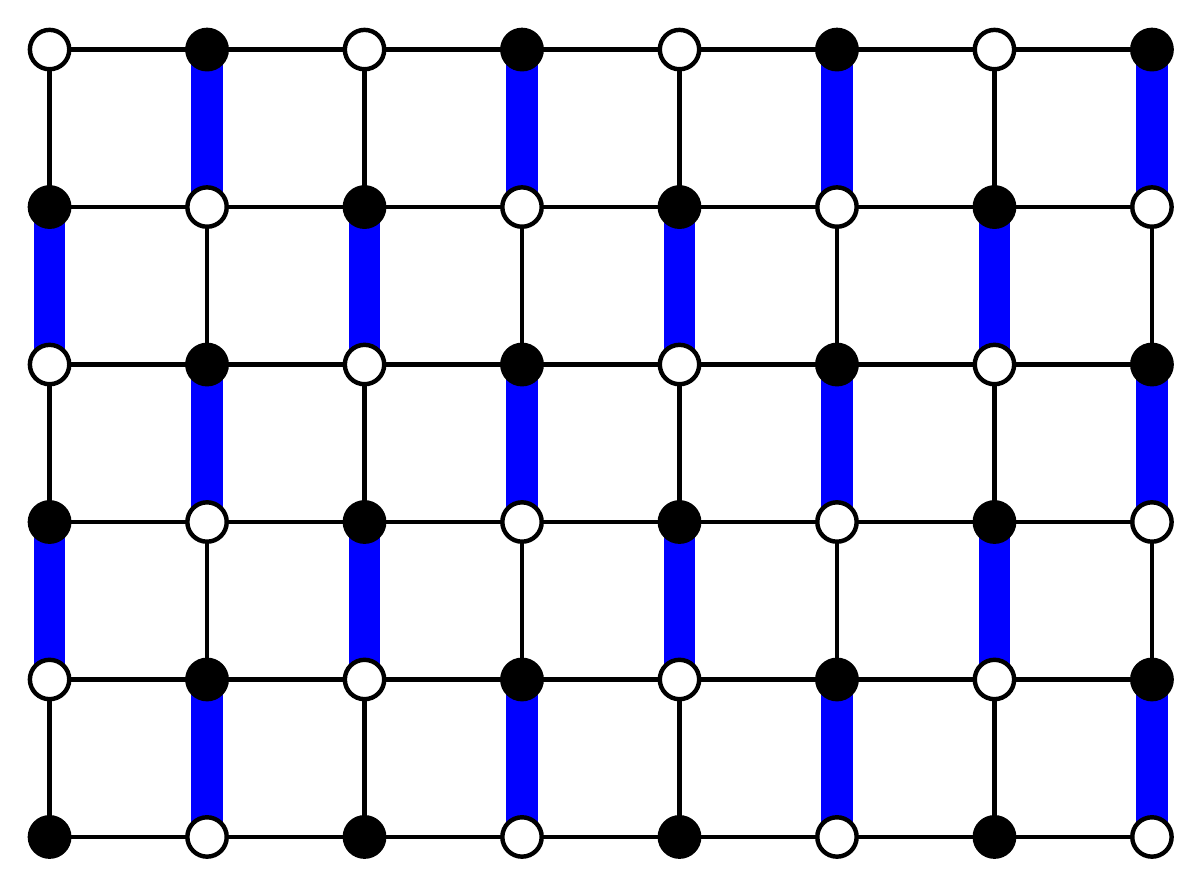
\begin{tikzpicture}
%vertex
\node (B1) at (0,0){$$}; \node (B2) at (4,0){$$}; \node (B3) at (8,0){$$}; \node (B4) at (12,0){$$}; 
\node (B5) at (2,2){$$}; \node (B6) at (6,2){$$}; \node (B7) at (10,2){$$}; \node (B8) at (14,2){$$}; 
\node (B9) at (0,4){$$}; \node (B10) at (4,4){$$}; \node (B11) at (8,4){$$}; \node (B12) at (12,4){$$}; 
\node (B13) at (2,6){$$}; \node (B14) at (6,6){$$}; \node (B15) at (10,6){$$}; \node (B16) at (14,6){$$};
\node (B17) at (0,8){$$}; \node (B18) at (4,8){$$}; \node (B19) at (8,8){$$}; \node (B20) at (12,8){$$}; 
\node (B21) at (2,10){$$}; \node (B22) at (6,10){$$}; \node (B23) at (10,10){$$}; \node (B24) at (14,10){$$};

\node (W1) at (2,0){$$}; \node (W2) at (6,0){$$}; \node (W3) at (10,0){$$}; \node (W4) at (14,0){$$}; 
\node (W5) at (0,2){$$}; \node (W6) at (4,2){$$}; \node (W7) at (8,2){$$}; \node (W8) at (12,2){$$};
\node (W9) at (2,4){$$}; \node (W10) at (6,4){$$}; \node (W11) at (10,4){$$}; \node (W12) at (14,4){$$}; 
\node (W13) at (0,6){$$}; \node (W14) at (4,6){$$}; \node (W15) at (8,6){$$}; \node (W16) at (12,6){$$};
\node (W17) at (2,8){$$}; \node (W18) at (6,8){$$}; \node (W19) at (10,8){$$}; \node (W20) at (14,8){$$}; 
\node (W21) at (0,10){$$}; \node (W22) at (4,10){$$}; \node (W23) at (8,10){$$}; \node (W24) at (12,10){$$};

%edge
\draw[line width=0.06cm] (B1)--(W1)--(B5)--(W5)--(B1); \draw[line width=0.06cm] (W1)--(B2)--(W6)--(B5)--(W1);
\draw[line width=0.06cm] (B2)--(W2)--(B6)--(W6)--(B2); \draw[line width=0.06cm] (W2)--(B3)--(W7)--(B6)--(W2);
\draw[line width=0.06cm] (B3)--(W3)--(B7)--(W7)--(B3); \draw[line width=0.06cm] (W3)--(B4)--(W8)--(B7)--(W3);
\draw[line width=0.06cm] (B4)--(W4)--(B8)--(W8)--(B4); 

\draw[line width=0.06cm] (W5)--(B5)--(W9)--(B9)--(W5); \draw[line width=0.06cm] (B5)--(W6)--(B10)--(W9)--(B5); 
\draw[line width=0.06cm] (W6)--(B6)--(W10)--(B10)--(W6); \draw[line width=0.06cm] (B6)--(W7)--(B11)--(W10)--(B6); 
\draw[line width=0.06cm] (W7)--(B7)--(W11)--(B11)--(W7); \draw[line width=0.06cm] (B7)--(W8)--(B12)--(W11)--(B7); 
\draw[line width=0.06cm] (W8)--(B8)--(W12)--(B12)--(W8); 

\draw[line width=0.06cm] (B9)--(W9)--(B13)--(W13)--(B9); \draw[line width=0.06cm] (W9)--(B10)--(W14)--(B13)--(W9);
\draw[line width=0.06cm] (B10)--(W10)--(B14)--(W14)--(B10); \draw[line width=0.06cm] (W10)--(B11)--(W15)--(B14)--(W10);
\draw[line width=0.06cm] (B11)--(W11)--(B15)--(W15)--(B11); \draw[line width=0.06cm] (W11)--(B12)--(W16)--(B15)--(W11);
\draw[line width=0.06cm] (B12)--(W12)--(B16)--(W16)--(B12); 

\draw[line width=0.06cm] (W13)--(B13)--(W17)--(B17)--(W13); \draw[line width=0.06cm] (B13)--(W14)--(B18)--(W17)--(B13); 
\draw[line width=0.06cm] (W14)--(B14)--(W18)--(B18)--(W14); \draw[line width=0.06cm] (B14)--(W15)--(B19)--(W18)--(B14); 
\draw[line width=0.06cm] (W15)--(B15)--(W19)--(B19)--(W15); \draw[line width=0.06cm] (B15)--(W16)--(B20)--(W19)--(B15); 
\draw[line width=0.06cm] (W16)--(B16)--(W20)--(B20)--(W16); 

\draw[line width=0.06cm] (B17)--(W17)--(B21)--(W21)--(B17); \draw[line width=0.06cm] (W17)--(B18)--(W22)--(B21)--(W17);
\draw[line width=0.06cm] (B18)--(W18)--(B22)--(W22)--(B18); \draw[line width=0.06cm] (W18)--(B19)--(W23)--(B22)--(W18);
\draw[line width=0.06cm] (B19)--(W19)--(B23)--(W23)--(B19); \draw[line width=0.06cm] (W19)--(B20)--(W24)--(B23)--(W19);
\draw[line width=0.06cm] (B20)--(W20)--(B24)--(W24)--(B20); 

%perfect matching
\draw[line width=0.4cm,color=blue] (W1)--(B5); \draw[line width=0.4cm,color=blue] (W2)--(B6); \draw[line width=0.4cm,color=blue] (W3)--(B7); 
\draw[line width=0.4cm,color=blue] (W4)--(B8); \draw[line width=0.4cm,color=blue] (W5)--(B9); \draw[line width=0.4cm,color=blue] (W6)--(B10); 
\draw[line width=0.4cm,color=blue] (W7)--(B11); \draw[line width=0.4cm,color=blue] (W8)--(B12); \draw[line width=0.4cm,color=blue] (W9)--(B13); 
\draw[line width=0.4cm,color=blue] (W10)--(B14); \draw[line width=0.4cm,color=blue] (W11)--(B15); \draw[line width=0.4cm,color=blue] (W12)--(B16); 
\draw[line width=0.4cm,color=blue] (W13)--(B17); \draw[line width=0.4cm,color=blue] (W14)--(B18); \draw[line width=0.4cm,color=blue] (W15)--(B19);
\draw[line width=0.4cm,color=blue] (W16)--(B20); \draw[line width=0.4cm,color=blue] (W17)--(B21); \draw[line width=0.4cm,color=blue] (W18)--(B22); 
\draw[line width=0.4cm,color=blue] (W19)--(B23); \draw[line width=0.4cm,color=blue] (W20)--(B24); 

%black
\filldraw [ultra thick, fill=black] (0,0) circle [radius=0.25] ; \filldraw [ultra thick, fill=black] (4,0) circle [radius=0.25] ;
\filldraw [ultra thick, fill=black] (8,0) circle [radius=0.25] ; \filldraw [ultra thick, fill=black] (12,0) circle [radius=0.25] ; 
\filldraw [ultra thick, fill=black] (2,2) circle [radius=0.25] ; \filldraw [ultra thick, fill=black] (6,2) circle [radius=0.25] ;
\filldraw [ultra thick, fill=black] (10,2) circle [radius=0.25] ; \filldraw [ultra thick, fill=black] (14,2) circle [radius=0.25] ;

\filldraw [ultra thick, fill=black] (0,4) circle [radius=0.25] ; \filldraw [ultra thick, fill=black] (4,4) circle [radius=0.25] ;
\filldraw [ultra thick, fill=black] (8,4) circle [radius=0.25] ; \filldraw [ultra thick, fill=black] (12,4) circle [radius=0.25] ;
\filldraw [ultra thick, fill=black] (2,6) circle [radius=0.25] ; \filldraw [ultra thick, fill=black] (6,6) circle [radius=0.25] ;
\filldraw [ultra thick, fill=black] (10,6) circle [radius=0.25] ; \filldraw [ultra thick, fill=black] (14,6) circle [radius=0.25] ;

\filldraw [ultra thick, fill=black] (0,8) circle [radius=0.25] ; \filldraw [ultra thick, fill=black] (4,8) circle [radius=0.25] ;
\filldraw [ultra thick, fill=black] (8,8) circle [radius=0.25] ; \filldraw [ultra thick, fill=black] (12,8) circle [radius=0.25] ;
\filldraw [ultra thick, fill=black] (2,10) circle [radius=0.25] ; \filldraw [ultra thick, fill=black] (6,10) circle [radius=0.25] ;
\filldraw [ultra thick, fill=black] (10,10) circle [radius=0.25] ; \filldraw [ultra thick, fill=black] (14,10) circle [radius=0.25] ;

%white
\filldraw [ultra thick, fill=white] (2,0) circle [radius=0.25] ; \filldraw [ultra thick, fill=white] (6,0) circle [radius=0.25] ;
\filldraw [ultra thick, fill=white] (10,0) circle [radius=0.25] ; \filldraw [ultra thick, fill=white] (14,0) circle [radius=0.25] ;
\filldraw [ultra thick, fill=white] (0,2) circle [radius=0.25] ; \filldraw [ultra thick, fill=white] (4,2) circle [radius=0.25] ;
\filldraw [ultra thick, fill=white] (8,2) circle [radius=0.25] ; \filldraw [ultra thick, fill=white] (12,2) circle [radius=0.25] ;

\filldraw [ultra thick, fill=white] (2,4) circle [radius=0.25] ; \filldraw [ultra thick, fill=white] (6,4) circle [radius=0.25] ;
\filldraw [ultra thick, fill=white] (10,4) circle [radius=0.25] ; \filldraw [ultra thick, fill=white] (14,4) circle [radius=0.25] ;
\filldraw [ultra thick, fill=white] (0,6) circle [radius=0.25] ; \filldraw [ultra thick, fill=white] (4,6) circle [radius=0.25] ;
\filldraw [ultra thick, fill=white] (8,6) circle [radius=0.25] ; \filldraw [ultra thick, fill=white] (12,6) circle [radius=0.25] ;

\filldraw [ultra thick, fill=white] (2,8) circle [radius=0.25] ; \filldraw [ultra thick, fill=white] (6,8) circle [radius=0.25] ;
\filldraw [ultra thick, fill=white] (10,8) circle [radius=0.25] ; \filldraw [ultra thick, fill=white] (14,8) circle [radius=0.25] ;
\filldraw [ultra thick, fill=white] (0,10) circle [radius=0.25] ; \filldraw [ultra thick, fill=white] (4,10) circle [radius=0.25] ;
\filldraw [ultra thick, fill=white] (8,10) circle [radius=0.25] ; \filldraw [ultra thick, fill=white] (12,10) circle [radius=0.25] ;
\end{tikzpicture}
} }; 

\node (PM3) at (0,-4.2) 
{\scalebox{0.3}{
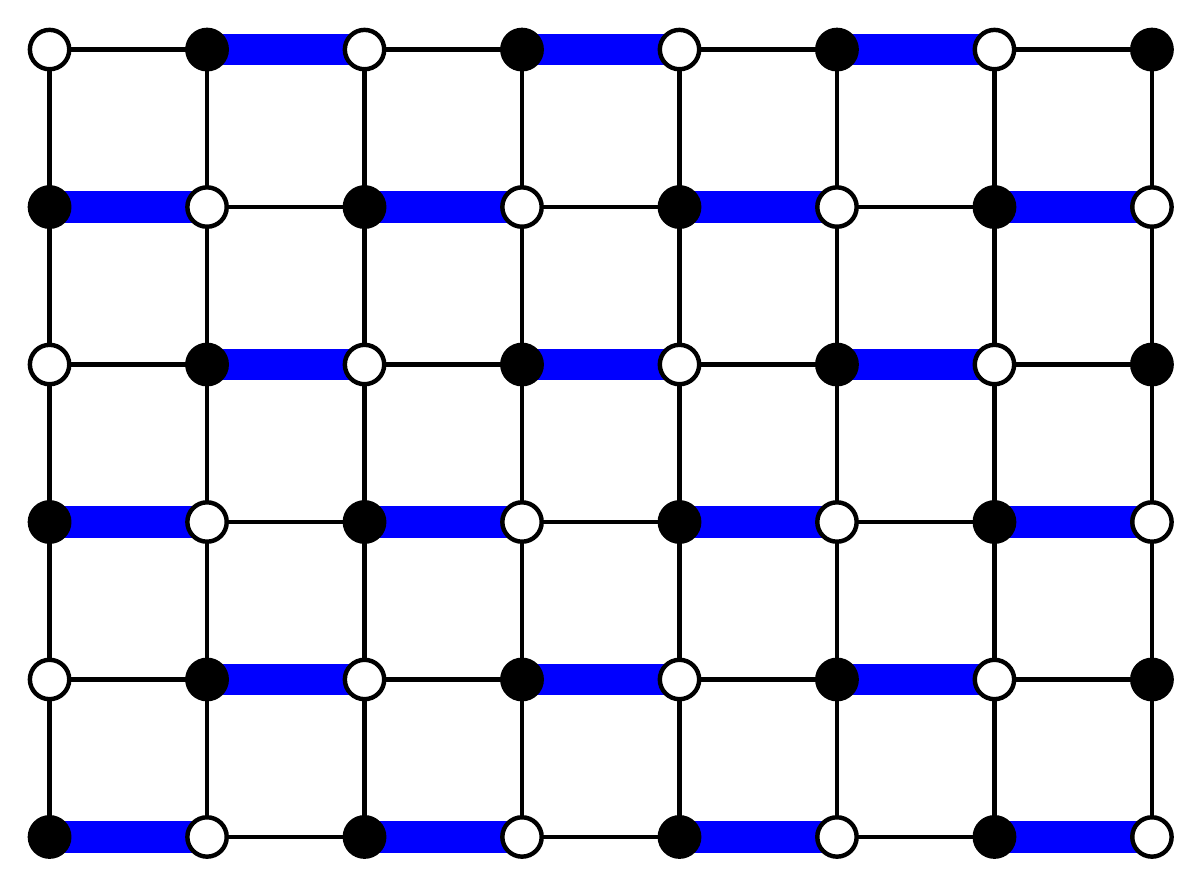
\begin{tikzpicture}
%vertex
\node (B1) at (0,0){$$}; \node (B2) at (4,0){$$}; \node (B3) at (8,0){$$}; \node (B4) at (12,0){$$}; 
\node (B5) at (2,2){$$}; \node (B6) at (6,2){$$}; \node (B7) at (10,2){$$}; \node (B8) at (14,2){$$}; 
\node (B9) at (0,4){$$}; \node (B10) at (4,4){$$}; \node (B11) at (8,4){$$}; \node (B12) at (12,4){$$}; 
\node (B13) at (2,6){$$}; \node (B14) at (6,6){$$}; \node (B15) at (10,6){$$}; \node (B16) at (14,6){$$};
\node (B17) at (0,8){$$}; \node (B18) at (4,8){$$}; \node (B19) at (8,8){$$}; \node (B20) at (12,8){$$}; 
\node (B21) at (2,10){$$}; \node (B22) at (6,10){$$}; \node (B23) at (10,10){$$}; \node (B24) at (14,10){$$};

\node (W1) at (2,0){$$}; \node (W2) at (6,0){$$}; \node (W3) at (10,0){$$}; \node (W4) at (14,0){$$}; 
\node (W5) at (0,2){$$}; \node (W6) at (4,2){$$}; \node (W7) at (8,2){$$}; \node (W8) at (12,2){$$};
\node (W9) at (2,4){$$}; \node (W10) at (6,4){$$}; \node (W11) at (10,4){$$}; \node (W12) at (14,4){$$}; 
\node (W13) at (0,6){$$}; \node (W14) at (4,6){$$}; \node (W15) at (8,6){$$}; \node (W16) at (12,6){$$};
\node (W17) at (2,8){$$}; \node (W18) at (6,8){$$}; \node (W19) at (10,8){$$}; \node (W20) at (14,8){$$}; 
\node (W21) at (0,10){$$}; \node (W22) at (4,10){$$}; \node (W23) at (8,10){$$}; \node (W24) at (12,10){$$};

%edge
\draw[line width=0.06cm] (B1)--(W1)--(B5)--(W5)--(B1); \draw[line width=0.06cm] (W1)--(B2)--(W6)--(B5)--(W1);
\draw[line width=0.06cm] (B2)--(W2)--(B6)--(W6)--(B2); \draw[line width=0.06cm] (W2)--(B3)--(W7)--(B6)--(W2);
\draw[line width=0.06cm] (B3)--(W3)--(B7)--(W7)--(B3); \draw[line width=0.06cm] (W3)--(B4)--(W8)--(B7)--(W3);
\draw[line width=0.06cm] (B4)--(W4)--(B8)--(W8)--(B4); 

\draw[line width=0.06cm] (W5)--(B5)--(W9)--(B9)--(W5); \draw[line width=0.06cm] (B5)--(W6)--(B10)--(W9)--(B5); 
\draw[line width=0.06cm] (W6)--(B6)--(W10)--(B10)--(W6); \draw[line width=0.06cm] (B6)--(W7)--(B11)--(W10)--(B6); 
\draw[line width=0.06cm] (W7)--(B7)--(W11)--(B11)--(W7); \draw[line width=0.06cm] (B7)--(W8)--(B12)--(W11)--(B7); 
\draw[line width=0.06cm] (W8)--(B8)--(W12)--(B12)--(W8); 

\draw[line width=0.06cm] (B9)--(W9)--(B13)--(W13)--(B9); \draw[line width=0.06cm] (W9)--(B10)--(W14)--(B13)--(W9);
\draw[line width=0.06cm] (B10)--(W10)--(B14)--(W14)--(B10); \draw[line width=0.06cm] (W10)--(B11)--(W15)--(B14)--(W10);
\draw[line width=0.06cm] (B11)--(W11)--(B15)--(W15)--(B11); \draw[line width=0.06cm] (W11)--(B12)--(W16)--(B15)--(W11);
\draw[line width=0.06cm] (B12)--(W12)--(B16)--(W16)--(B12); 

\draw[line width=0.06cm] (W13)--(B13)--(W17)--(B17)--(W13); \draw[line width=0.06cm] (B13)--(W14)--(B18)--(W17)--(B13); 
\draw[line width=0.06cm] (W14)--(B14)--(W18)--(B18)--(W14); \draw[line width=0.06cm] (B14)--(W15)--(B19)--(W18)--(B14); 
\draw[line width=0.06cm] (W15)--(B15)--(W19)--(B19)--(W15); \draw[line width=0.06cm] (B15)--(W16)--(B20)--(W19)--(B15); 
\draw[line width=0.06cm] (W16)--(B16)--(W20)--(B20)--(W16); 

\draw[line width=0.06cm] (B17)--(W17)--(B21)--(W21)--(B17); \draw[line width=0.06cm] (W17)--(B18)--(W22)--(B21)--(W17);
\draw[line width=0.06cm] (B18)--(W18)--(B22)--(W22)--(B18); \draw[line width=0.06cm] (W18)--(B19)--(W23)--(B22)--(W18);
\draw[line width=0.06cm] (B19)--(W19)--(B23)--(W23)--(B19); \draw[line width=0.06cm] (W19)--(B20)--(W24)--(B23)--(W19);
\draw[line width=0.06cm] (B20)--(W20)--(B24)--(W24)--(B20); 

%perfect matching
\draw[line width=0.4cm,color=blue] (B1)--(W1); \draw[line width=0.4cm,color=blue] (B2)--(W2); 
\draw[line width=0.4cm,color=blue] (B3)--(W3); \draw[line width=0.4cm,color=blue] (B4)--(W4); 
\draw[line width=0.4cm,color=blue] (B5)--(W6); \draw[line width=0.4cm,color=blue] (B6)--(W7); 
\draw[line width=0.4cm,color=blue] (B7)--(W8); 
\draw[line width=0.4cm,color=blue] (B9)--(W9); \draw[line width=0.4cm,color=blue] (B10)--(W10); 
\draw[line width=0.4cm,color=blue] (B11)--(W11); \draw[line width=0.4cm,color=blue] (B12)--(W12); 
\draw[line width=0.4cm,color=blue] (B13)--(W14); \draw[line width=0.4cm,color=blue] (B14)--(W15); 
\draw[line width=0.4cm,color=blue] (B15)--(W16); \draw[line width=0.4cm,color=blue] (B17)--(W17); 
\draw[line width=0.4cm,color=blue] (B18)--(W18); \draw[line width=0.4cm,color=blue] (B19)--(W19); 
\draw[line width=0.4cm,color=blue] (B20)--(W20); 
\draw[line width=0.4cm,color=blue] (B21)--(W22); \draw[line width=0.4cm,color=blue] (B22)--(W23); 
\draw[line width=0.4cm,color=blue] (B23)--(W24);

%black
\filldraw [ultra thick, fill=black] (0,0) circle [radius=0.25] ; \filldraw [ultra thick, fill=black] (4,0) circle [radius=0.25] ;
\filldraw [ultra thick, fill=black] (8,0) circle [radius=0.25] ; \filldraw [ultra thick, fill=black] (12,0) circle [radius=0.25] ; 
\filldraw [ultra thick, fill=black] (2,2) circle [radius=0.25] ; \filldraw [ultra thick, fill=black] (6,2) circle [radius=0.25] ;
\filldraw [ultra thick, fill=black] (10,2) circle [radius=0.25] ; \filldraw [ultra thick, fill=black] (14,2) circle [radius=0.25] ;

\filldraw [ultra thick, fill=black] (0,4) circle [radius=0.25] ; \filldraw [ultra thick, fill=black] (4,4) circle [radius=0.25] ;
\filldraw [ultra thick, fill=black] (8,4) circle [radius=0.25] ; \filldraw [ultra thick, fill=black] (12,4) circle [radius=0.25] ;
\filldraw [ultra thick, fill=black] (2,6) circle [radius=0.25] ; \filldraw [ultra thick, fill=black] (6,6) circle [radius=0.25] ;
\filldraw [ultra thick, fill=black] (10,6) circle [radius=0.25] ; \filldraw [ultra thick, fill=black] (14,6) circle [radius=0.25] ;

\filldraw [ultra thick, fill=black] (0,8) circle [radius=0.25] ; \filldraw [ultra thick, fill=black] (4,8) circle [radius=0.25] ;
\filldraw [ultra thick, fill=black] (8,8) circle [radius=0.25] ; \filldraw [ultra thick, fill=black] (12,8) circle [radius=0.25] ;
\filldraw [ultra thick, fill=black] (2,10) circle [radius=0.25] ; \filldraw [ultra thick, fill=black] (6,10) circle [radius=0.25] ;
\filldraw [ultra thick, fill=black] (10,10) circle [radius=0.25] ; \filldraw [ultra thick, fill=black] (14,10) circle [radius=0.25] ;

%white
\filldraw [ultra thick, fill=white] (2,0) circle [radius=0.25] ; \filldraw [ultra thick, fill=white] (6,0) circle [radius=0.25] ;
\filldraw [ultra thick, fill=white] (10,0) circle [radius=0.25] ; \filldraw [ultra thick, fill=white] (14,0) circle [radius=0.25] ;
\filldraw [ultra thick, fill=white] (0,2) circle [radius=0.25] ; \filldraw [ultra thick, fill=white] (4,2) circle [radius=0.25] ;
\filldraw [ultra thick, fill=white] (8,2) circle [radius=0.25] ; \filldraw [ultra thick, fill=white] (12,2) circle [radius=0.25] ;

\filldraw [ultra thick, fill=white] (2,4) circle [radius=0.25] ; \filldraw [ultra thick, fill=white] (6,4) circle [radius=0.25] ;
\filldraw [ultra thick, fill=white] (10,4) circle [radius=0.25] ; \filldraw [ultra thick, fill=white] (14,4) circle [radius=0.25] ;
\filldraw [ultra thick, fill=white] (0,6) circle [radius=0.25] ; \filldraw [ultra thick, fill=white] (4,6) circle [radius=0.25] ;
\filldraw [ultra thick, fill=white] (8,6) circle [radius=0.25] ; \filldraw [ultra thick, fill=white] (12,6) circle [radius=0.25] ;

\filldraw [ultra thick, fill=white] (2,8) circle [radius=0.25] ; \filldraw [ultra thick, fill=white] (6,8) circle [radius=0.25] ;
\filldraw [ultra thick, fill=white] (10,8) circle [radius=0.25] ; \filldraw [ultra thick, fill=white] (14,8) circle [radius=0.25] ;
\filldraw [ultra thick, fill=white] (0,10) circle [radius=0.25] ; \filldraw [ultra thick, fill=white] (4,10) circle [radius=0.25] ;
\filldraw [ultra thick, fill=white] (8,10) circle [radius=0.25] ; \filldraw [ultra thick, fill=white] (12,10) circle [radius=0.25] ;
\end{tikzpicture}
} }; 

\node (PM4) at (6,-4.2) 
{\scalebox{0.3}{
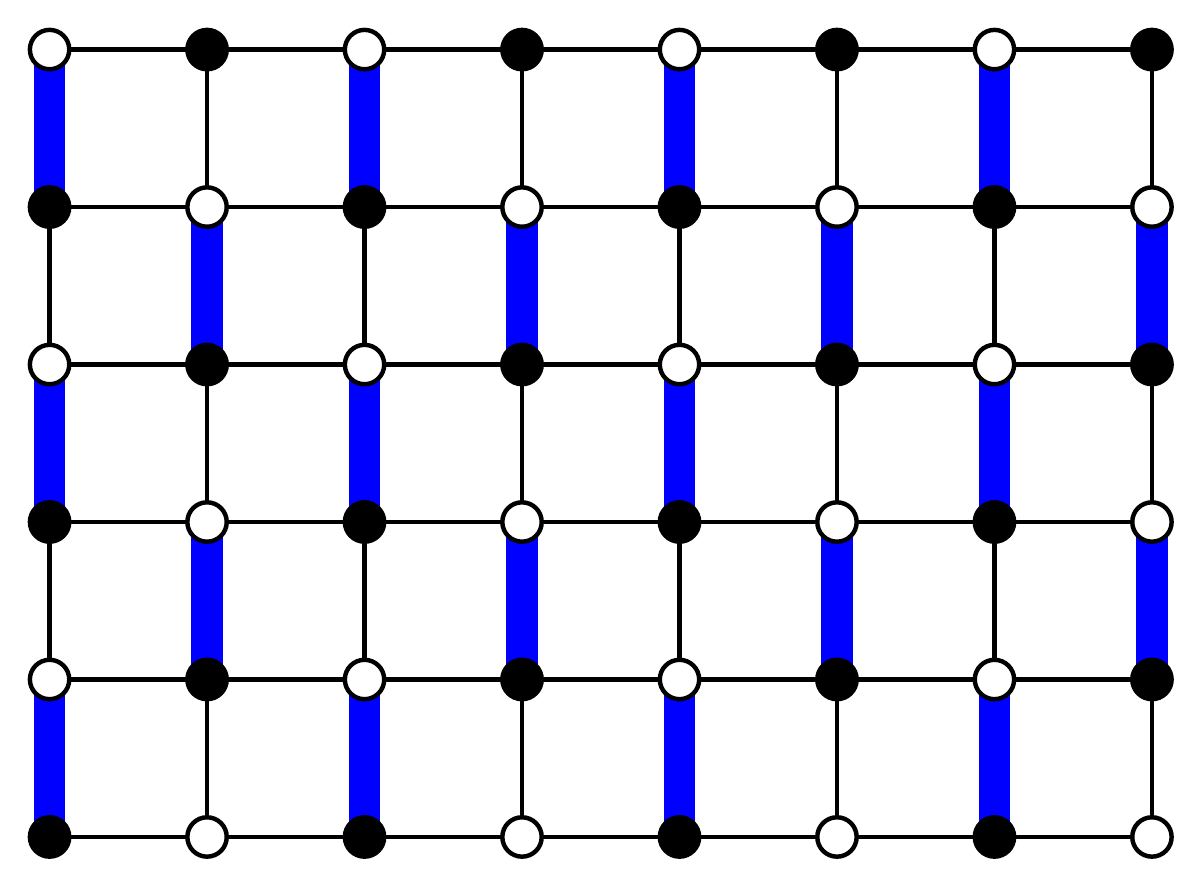
\begin{tikzpicture}
%vertex
\node (B1) at (0,0){$$}; \node (B2) at (4,0){$$}; \node (B3) at (8,0){$$}; \node (B4) at (12,0){$$}; 
\node (B5) at (2,2){$$}; \node (B6) at (6,2){$$}; \node (B7) at (10,2){$$}; \node (B8) at (14,2){$$}; 
\node (B9) at (0,4){$$}; \node (B10) at (4,4){$$}; \node (B11) at (8,4){$$}; \node (B12) at (12,4){$$}; 
\node (B13) at (2,6){$$}; \node (B14) at (6,6){$$}; \node (B15) at (10,6){$$}; \node (B16) at (14,6){$$};
\node (B17) at (0,8){$$}; \node (B18) at (4,8){$$}; \node (B19) at (8,8){$$}; \node (B20) at (12,8){$$}; 
\node (B21) at (2,10){$$}; \node (B22) at (6,10){$$}; \node (B23) at (10,10){$$}; \node (B24) at (14,10){$$};

\node (W1) at (2,0){$$}; \node (W2) at (6,0){$$}; \node (W3) at (10,0){$$}; \node (W4) at (14,0){$$}; 
\node (W5) at (0,2){$$}; \node (W6) at (4,2){$$}; \node (W7) at (8,2){$$}; \node (W8) at (12,2){$$};
\node (W9) at (2,4){$$}; \node (W10) at (6,4){$$}; \node (W11) at (10,4){$$}; \node (W12) at (14,4){$$}; 
\node (W13) at (0,6){$$}; \node (W14) at (4,6){$$}; \node (W15) at (8,6){$$}; \node (W16) at (12,6){$$};
\node (W17) at (2,8){$$}; \node (W18) at (6,8){$$}; \node (W19) at (10,8){$$}; \node (W20) at (14,8){$$}; 
\node (W21) at (0,10){$$}; \node (W22) at (4,10){$$}; \node (W23) at (8,10){$$}; \node (W24) at (12,10){$$};

%edge
\draw[line width=0.06cm] (B1)--(W1)--(B5)--(W5)--(B1); \draw[line width=0.06cm] (W1)--(B2)--(W6)--(B5)--(W1);
\draw[line width=0.06cm] (B2)--(W2)--(B6)--(W6)--(B2); \draw[line width=0.06cm] (W2)--(B3)--(W7)--(B6)--(W2);
\draw[line width=0.06cm] (B3)--(W3)--(B7)--(W7)--(B3); \draw[line width=0.06cm] (W3)--(B4)--(W8)--(B7)--(W3);
\draw[line width=0.06cm] (B4)--(W4)--(B8)--(W8)--(B4); 

\draw[line width=0.06cm] (W5)--(B5)--(W9)--(B9)--(W5); \draw[line width=0.06cm] (B5)--(W6)--(B10)--(W9)--(B5); 
\draw[line width=0.06cm] (W6)--(B6)--(W10)--(B10)--(W6); \draw[line width=0.06cm] (B6)--(W7)--(B11)--(W10)--(B6); 
\draw[line width=0.06cm] (W7)--(B7)--(W11)--(B11)--(W7); \draw[line width=0.06cm] (B7)--(W8)--(B12)--(W11)--(B7); 
\draw[line width=0.06cm] (W8)--(B8)--(W12)--(B12)--(W8); 

\draw[line width=0.06cm] (B9)--(W9)--(B13)--(W13)--(B9); \draw[line width=0.06cm] (W9)--(B10)--(W14)--(B13)--(W9);
\draw[line width=0.06cm] (B10)--(W10)--(B14)--(W14)--(B10); \draw[line width=0.06cm] (W10)--(B11)--(W15)--(B14)--(W10);
\draw[line width=0.06cm] (B11)--(W11)--(B15)--(W15)--(B11); \draw[line width=0.06cm] (W11)--(B12)--(W16)--(B15)--(W11);
\draw[line width=0.06cm] (B12)--(W12)--(B16)--(W16)--(B12); 

\draw[line width=0.06cm] (W13)--(B13)--(W17)--(B17)--(W13); \draw[line width=0.06cm] (B13)--(W14)--(B18)--(W17)--(B13); 
\draw[line width=0.06cm] (W14)--(B14)--(W18)--(B18)--(W14); \draw[line width=0.06cm] (B14)--(W15)--(B19)--(W18)--(B14); 
\draw[line width=0.06cm] (W15)--(B15)--(W19)--(B19)--(W15); \draw[line width=0.06cm] (B15)--(W16)--(B20)--(W19)--(B15); 
\draw[line width=0.06cm] (W16)--(B16)--(W20)--(B20)--(W16); 

\draw[line width=0.06cm] (B17)--(W17)--(B21)--(W21)--(B17); \draw[line width=0.06cm] (W17)--(B18)--(W22)--(B21)--(W17);
\draw[line width=0.06cm] (B18)--(W18)--(B22)--(W22)--(B18); \draw[line width=0.06cm] (W18)--(B19)--(W23)--(B22)--(W18);
\draw[line width=0.06cm] (B19)--(W19)--(B23)--(W23)--(B19); \draw[line width=0.06cm] (W19)--(B20)--(W24)--(B23)--(W19);
\draw[line width=0.06cm] (B20)--(W20)--(B24)--(W24)--(B20); 

%perfect matching 
\draw[line width=0.4cm,color=blue] (W5)--(B1); \draw[line width=0.4cm,color=blue] (W6)--(B2); \draw[line width=0.4cm,color=blue] (W7)--(B3); 
\draw[line width=0.4cm,color=blue] (W8)--(B4); \draw[line width=0.4cm,color=blue] (W9)--(B5); \draw[line width=0.4cm,color=blue] (W10)--(B6); 
\draw[line width=0.4cm,color=blue] (W11)--(B7); \draw[line width=0.4cm,color=blue] (W12)--(B8); \draw[line width=0.4cm,color=blue] (W13)--(B9); 
\draw[line width=0.4cm,color=blue] (W14)--(B10); \draw[line width=0.4cm,color=blue] (W15)--(B11); \draw[line width=0.4cm,color=blue] (W16)--(B12); 
\draw[line width=0.4cm,color=blue] (W17)--(B13); \draw[line width=0.4cm,color=blue] (W18)--(B14); \draw[line width=0.4cm,color=blue] (W19)--(B15); 
\draw[line width=0.4cm,color=blue] (W20)--(B16); \draw[line width=0.4cm,color=blue] (W21)--(B17); \draw[line width=0.4cm,color=blue] (W22)--(B18); 
\draw[line width=0.4cm,color=blue] (W23)--(B19); \draw[line width=0.4cm,color=blue] (W24)--(B20); 

%black
\filldraw [ultra thick, fill=black] (0,0) circle [radius=0.25] ; \filldraw [ultra thick, fill=black] (4,0) circle [radius=0.25] ;
\filldraw [ultra thick, fill=black] (8,0) circle [radius=0.25] ; \filldraw [ultra thick, fill=black] (12,0) circle [radius=0.25] ; 
\filldraw [ultra thick, fill=black] (2,2) circle [radius=0.25] ; \filldraw [ultra thick, fill=black] (6,2) circle [radius=0.25] ;
\filldraw [ultra thick, fill=black] (10,2) circle [radius=0.25] ; \filldraw [ultra thick, fill=black] (14,2) circle [radius=0.25] ;

\filldraw [ultra thick, fill=black] (0,4) circle [radius=0.25] ; \filldraw [ultra thick, fill=black] (4,4) circle [radius=0.25] ;
\filldraw [ultra thick, fill=black] (8,4) circle [radius=0.25] ; \filldraw [ultra thick, fill=black] (12,4) circle [radius=0.25] ;
\filldraw [ultra thick, fill=black] (2,6) circle [radius=0.25] ; \filldraw [ultra thick, fill=black] (6,6) circle [radius=0.25] ;
\filldraw [ultra thick, fill=black] (10,6) circle [radius=0.25] ; \filldraw [ultra thick, fill=black] (14,6) circle [radius=0.25] ;

\filldraw [ultra thick, fill=black] (0,8) circle [radius=0.25] ; \filldraw [ultra thick, fill=black] (4,8) circle [radius=0.25] ;
\filldraw [ultra thick, fill=black] (8,8) circle [radius=0.25] ; \filldraw [ultra thick, fill=black] (12,8) circle [radius=0.25] ;
\filldraw [ultra thick, fill=black] (2,10) circle [radius=0.25] ; \filldraw [ultra thick, fill=black] (6,10) circle [radius=0.25] ;
\filldraw [ultra thick, fill=black] (10,10) circle [radius=0.25] ; \filldraw [ultra thick, fill=black] (14,10) circle [radius=0.25] ;

%white
\filldraw [ultra thick, fill=white] (2,0) circle [radius=0.25] ; \filldraw [ultra thick, fill=white] (6,0) circle [radius=0.25] ;
\filldraw [ultra thick, fill=white] (10,0) circle [radius=0.25] ; \filldraw [ultra thick, fill=white] (14,0) circle [radius=0.25] ;
\filldraw [ultra thick, fill=white] (0,2) circle [radius=0.25] ; \filldraw [ultra thick, fill=white] (4,2) circle [radius=0.25] ;
\filldraw [ultra thick, fill=white] (8,2) circle [radius=0.25] ; \filldraw [ultra thick, fill=white] (12,2) circle [radius=0.25] ;

\filldraw [ultra thick, fill=white] (2,4) circle [radius=0.25] ; \filldraw [ultra thick, fill=white] (6,4) circle [radius=0.25] ;
\filldraw [ultra thick, fill=white] (10,4) circle [radius=0.25] ; \filldraw [ultra thick, fill=white] (14,4) circle [radius=0.25] ;
\filldraw [ultra thick, fill=white] (0,6) circle [radius=0.25] ; \filldraw [ultra thick, fill=white] (4,6) circle [radius=0.25] ;
\filldraw [ultra thick, fill=white] (8,6) circle [radius=0.25] ; \filldraw [ultra thick, fill=white] (12,6) circle [radius=0.25] ;

\filldraw [ultra thick, fill=white] (2,8) circle [radius=0.25] ; \filldraw [ultra thick, fill=white] (6,8) circle [radius=0.25] ;
\filldraw [ultra thick, fill=white] (10,8) circle [radius=0.25] ; \filldraw [ultra thick, fill=white] (14,8) circle [radius=0.25] ;
\filldraw [ultra thick, fill=white] (0,10) circle [radius=0.25] ; \filldraw [ultra thick, fill=white] (4,10) circle [radius=0.25] ;
\filldraw [ultra thick, fill=white] (8,10) circle [radius=0.25] ; \filldraw [ultra thick, fill=white] (12,10) circle [radius=0.25] ;
\end{tikzpicture}
} }; 

\end{tikzpicture}
}}
\caption{Extremal perfect matchings of a square dimer model}
\label{expm_square}
\end{figure}

\begin{figure}[htb]
\centering
\begin{tabular}{c}
\begin{minipage}{0.45\hsize}\centering
%\begin{center}
{\scalebox{0.35}{
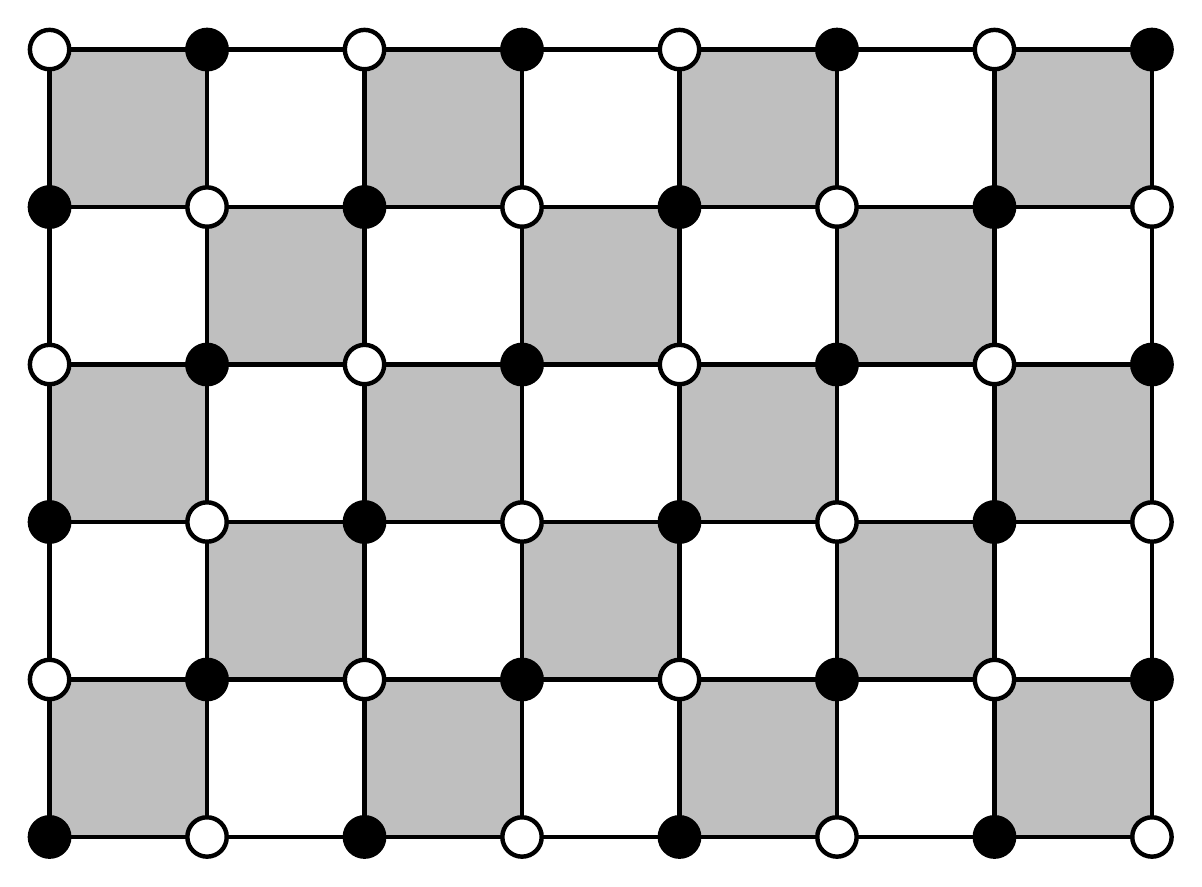
\begin{tikzpicture}
%vertex
\node (B1) at (0,0){$$}; \node (B2) at (4,0){$$}; \node (B3) at (8,0){$$}; \node (B4) at (12,0){$$}; 
\node (B5) at (2,2){$$}; \node (B6) at (6,2){$$}; \node (B7) at (10,2){$$}; \node (B8) at (14,2){$$}; 
\node (B9) at (0,4){$$}; \node (B10) at (4,4){$$}; \node (B11) at (8,4){$$}; \node (B12) at (12,4){$$}; 
\node (B13) at (2,6){$$}; \node (B14) at (6,6){$$}; \node (B15) at (10,6){$$}; \node (B16) at (14,6){$$};
\node (B17) at (0,8){$$}; \node (B18) at (4,8){$$}; \node (B19) at (8,8){$$}; \node (B20) at (12,8){$$}; 
\node (B21) at (2,10){$$}; \node (B22) at (6,10){$$}; \node (B23) at (10,10){$$}; \node (B24) at (14,10){$$};

\node (W1) at (2,0){$$}; \node (W2) at (6,0){$$}; \node (W3) at (10,0){$$}; \node (W4) at (14,0){$$}; 
\node (W5) at (0,2){$$}; \node (W6) at (4,2){$$}; \node (W7) at (8,2){$$}; \node (W8) at (12,2){$$};
\node (W9) at (2,4){$$}; \node (W10) at (6,4){$$}; \node (W11) at (10,4){$$}; \node (W12) at (14,4){$$}; 
\node (W13) at (0,6){$$}; \node (W14) at (4,6){$$}; \node (W15) at (8,6){$$}; \node (W16) at (12,6){$$};
\node (W17) at (2,8){$$}; \node (W18) at (6,8){$$}; \node (W19) at (10,8){$$}; \node (W20) at (14,8){$$}; 
\node (W21) at (0,10){$$}; \node (W22) at (4,10){$$}; \node (W23) at (8,10){$$}; \node (W24) at (12,10){$$};


\draw [fill=lightgray] (B1) rectangle (B5); \draw [fill=lightgray] (B2) rectangle (B6); \draw [fill=lightgray] (B3) rectangle (B7); \draw [fill=lightgray] (B4) rectangle (B8); 
\draw [fill=lightgray] (B5) rectangle (B10); \draw [fill=lightgray] (B6) rectangle (B11); \draw [fill=lightgray] (B7) rectangle (B12); 
\draw [fill=lightgray] (B9) rectangle (B13); \draw [fill=lightgray] (B10) rectangle (B14); \draw [fill=lightgray] (B11) rectangle (B15); \draw [fill=lightgray] (B12) rectangle (B16); 
\draw [fill=lightgray] (B13) rectangle (B18); \draw [fill=lightgray] (B14) rectangle (B19); \draw [fill=lightgray] (B15) rectangle (B20); 
\draw [fill=lightgray] (B17) rectangle (B21); \draw [fill=lightgray] (B18) rectangle (B22); \draw [fill=lightgray] (B19) rectangle (B23); 
\draw [fill=lightgray] (B20) rectangle (B24); 

%edge
\draw[line width=0.06cm] (B1)--(W1)--(B5)--(W5)--(B1); \draw[line width=0.06cm] (W1)--(B2)--(W6)--(B5)--(W1);
\draw[line width=0.06cm] (B2)--(W2)--(B6)--(W6)--(B2); \draw[line width=0.06cm] (W2)--(B3)--(W7)--(B6)--(W2);
\draw[line width=0.06cm] (B3)--(W3)--(B7)--(W7)--(B3); \draw[line width=0.06cm] (W3)--(B4)--(W8)--(B7)--(W3);
\draw[line width=0.06cm] (B4)--(W4)--(B8)--(W8)--(B4); 

\draw[line width=0.06cm] (W5)--(B5)--(W9)--(B9)--(W5); \draw[line width=0.06cm] (B5)--(W6)--(B10)--(W9)--(B5); 
\draw[line width=0.06cm] (W6)--(B6)--(W10)--(B10)--(W6); \draw[line width=0.06cm] (B6)--(W7)--(B11)--(W10)--(B6); 
\draw[line width=0.06cm] (W7)--(B7)--(W11)--(B11)--(W7); \draw[line width=0.06cm] (B7)--(W8)--(B12)--(W11)--(B7); 
\draw[line width=0.06cm] (W8)--(B8)--(W12)--(B12)--(W8); 

\draw[line width=0.06cm] (B9)--(W9)--(B13)--(W13)--(B9); \draw[line width=0.06cm] (W9)--(B10)--(W14)--(B13)--(W9);
\draw[line width=0.06cm] (B10)--(W10)--(B14)--(W14)--(B10); \draw[line width=0.06cm] (W10)--(B11)--(W15)--(B14)--(W10);
\draw[line width=0.06cm] (B11)--(W11)--(B15)--(W15)--(B11); \draw[line width=0.06cm] (W11)--(B12)--(W16)--(B15)--(W11);
\draw[line width=0.06cm] (B12)--(W12)--(B16)--(W16)--(B12); 

\draw[line width=0.06cm] (W13)--(B13)--(W17)--(B17)--(W13); \draw[line width=0.06cm] (B13)--(W14)--(B18)--(W17)--(B13); 
\draw[line width=0.06cm] (W14)--(B14)--(W18)--(B18)--(W14); \draw[line width=0.06cm] (B14)--(W15)--(B19)--(W18)--(B14); 
\draw[line width=0.06cm] (W15)--(B15)--(W19)--(B19)--(W15); \draw[line width=0.06cm] (B15)--(W16)--(B20)--(W19)--(B15); 
\draw[line width=0.06cm] (W16)--(B16)--(W20)--(B20)--(W16); 

\draw[line width=0.06cm] (B17)--(W17)--(B21)--(W21)--(B17); \draw[line width=0.06cm] (W17)--(B18)--(W22)--(B21)--(W17);
\draw[line width=0.06cm] (B18)--(W18)--(B22)--(W22)--(B18); \draw[line width=0.06cm] (W18)--(B19)--(W23)--(B22)--(W18);
\draw[line width=0.06cm] (B19)--(W19)--(B23)--(W23)--(B19); \draw[line width=0.06cm] (W19)--(B20)--(W24)--(B23)--(W19);
\draw[line width=0.06cm] (B20)--(W20)--(B24)--(W24)--(B20); 

%black
\filldraw [ultra thick, fill=black] (0,0) circle [radius=0.25] ; \filldraw [ultra thick, fill=black] (4,0) circle [radius=0.25] ;
\filldraw [ultra thick, fill=black] (8,0) circle [radius=0.25] ; \filldraw [ultra thick, fill=black] (12,0) circle [radius=0.25] ; 
\filldraw [ultra thick, fill=black] (2,2) circle [radius=0.25] ; \filldraw [ultra thick, fill=black] (6,2) circle [radius=0.25] ;
\filldraw [ultra thick, fill=black] (10,2) circle [radius=0.25] ; \filldraw [ultra thick, fill=black] (14,2) circle [radius=0.25] ;

\filldraw [ultra thick, fill=black] (0,4) circle [radius=0.25] ; \filldraw [ultra thick, fill=black] (4,4) circle [radius=0.25] ;
\filldraw [ultra thick, fill=black] (8,4) circle [radius=0.25] ; \filldraw [ultra thick, fill=black] (12,4) circle [radius=0.25] ;
\filldraw [ultra thick, fill=black] (2,6) circle [radius=0.25] ; \filldraw [ultra thick, fill=black] (6,6) circle [radius=0.25] ;
\filldraw [ultra thick, fill=black] (10,6) circle [radius=0.25] ; \filldraw [ultra thick, fill=black] (14,6) circle [radius=0.25] ;

\filldraw [ultra thick, fill=black] (0,8) circle [radius=0.25] ; \filldraw [ultra thick, fill=black] (4,8) circle [radius=0.25] ;
\filldraw [ultra thick, fill=black] (8,8) circle [radius=0.25] ; \filldraw [ultra thick, fill=black] (12,8) circle [radius=0.25] ;
\filldraw [ultra thick, fill=black] (2,10) circle [radius=0.25] ; \filldraw [ultra thick, fill=black] (6,10) circle [radius=0.25] ;
\filldraw [ultra thick, fill=black] (10,10) circle [radius=0.25] ; \filldraw [ultra thick, fill=black] (14,10) circle [radius=0.25] ;

%white
\filldraw [ultra thick, fill=white] (2,0) circle [radius=0.25] ; \filldraw [ultra thick, fill=white] (6,0) circle [radius=0.25] ;
\filldraw [ultra thick, fill=white] (10,0) circle [radius=0.25] ; \filldraw [ultra thick, fill=white] (14,0) circle [radius=0.25] ;
\filldraw [ultra thick, fill=white] (0,2) circle [radius=0.25] ; \filldraw [ultra thick, fill=white] (4,2) circle [radius=0.25] ;
\filldraw [ultra thick, fill=white] (8,2) circle [radius=0.25] ; \filldraw [ultra thick, fill=white] (12,2) circle [radius=0.25] ;

\filldraw [ultra thick, fill=white] (2,4) circle [radius=0.25] ; \filldraw [ultra thick, fill=white] (6,4) circle [radius=0.25] ;
\filldraw [ultra thick, fill=white] (10,4) circle [radius=0.25] ; \filldraw [ultra thick, fill=white] (14,4) circle [radius=0.25] ;
\filldraw [ultra thick, fill=white] (0,6) circle [radius=0.25] ; \filldraw [ultra thick, fill=white] (4,6) circle [radius=0.25] ;
\filldraw [ultra thick, fill=white] (8,6) circle [radius=0.25] ; \filldraw [ultra thick, fill=white] (12,6) circle [radius=0.25] ;

\filldraw [ultra thick, fill=white] (2,8) circle [radius=0.25] ; \filldraw [ultra thick, fill=white] (6,8) circle [radius=0.25] ;
\filldraw [ultra thick, fill=white] (10,8) circle [radius=0.25] ; \filldraw [ultra thick, fill=white] (14,8) circle [radius=0.25] ;
\filldraw [ultra thick, fill=white] (0,10) circle [radius=0.25] ; \filldraw [ultra thick, fill=white] (4,10) circle [radius=0.25] ;
\filldraw [ultra thick, fill=white] (8,10) circle [radius=0.25] ; \filldraw [ultra thick, fill=white] (12,10) circle [radius=0.25] ;

\end{tikzpicture} }}
%\end{center}
\caption{}
\label{faces_semisteady}
\end{minipage}


\begin{minipage}{0.45\hsize}\centering
%\begin{center}
{\scalebox{0.35}{
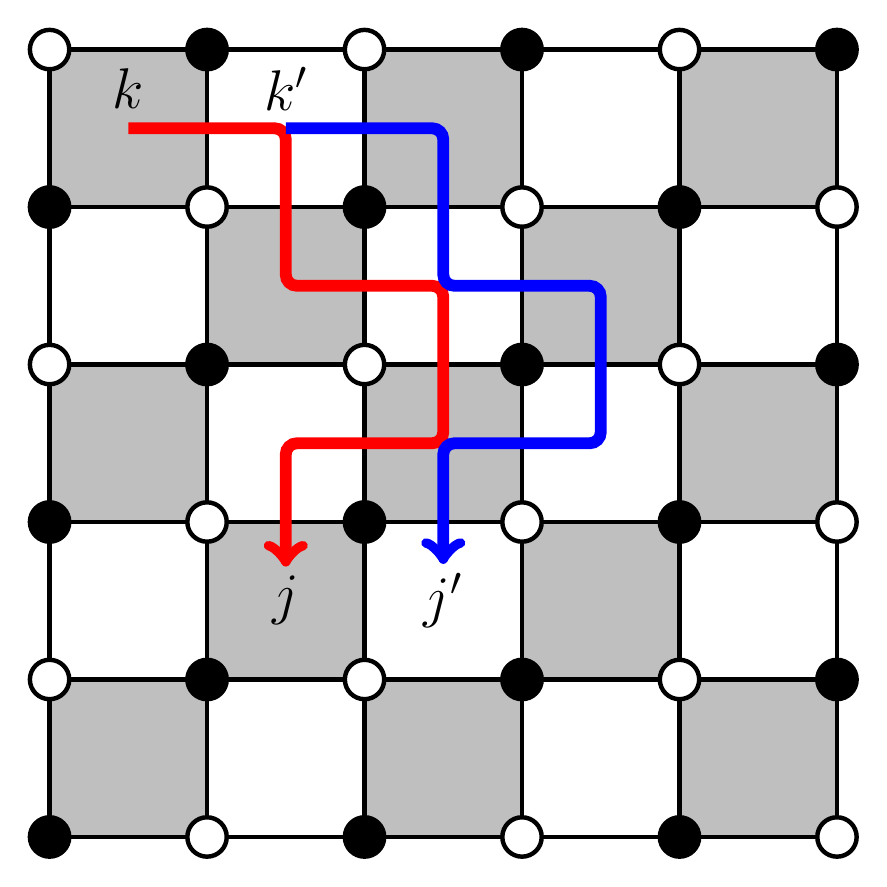
\begin{tikzpicture}
%vertex
\node (B1) at (0,0){$$}; \node (B2) at (4,0){$$}; \node (B3) at (8,0){$$}; 
\node (B5) at (2,2){$$}; \node (B6) at (6,2){$$}; \node (B7) at (10,2){$$}; 
\node (B9) at (0,4){$$}; \node (B10) at (4,4){$$}; \node (B11) at (8,4){$$}; 
\node (B13) at (2,6){$$}; \node (B14) at (6,6){$$}; \node (B15) at (10,6){$$}; 
\node (B17) at (0,8){$$}; \node (B18) at (4,8){$$}; \node (B19) at (8,8){$$}; 
\node (B21) at (2,10){$$}; \node (B22) at (6,10){$$}; \node (B23) at (10,10){$$}; 

\node (W1) at (2,0){$$}; \node (W2) at (6,0){$$}; \node (W3) at (10,0){$$};
\node (W5) at (0,2){$$}; \node (W6) at (4,2){$$}; \node (W7) at (8,2){$$}; 
\node (W9) at (2,4){$$}; \node (W10) at (6,4){$$}; \node (W11) at (10,4){$$}; 
\node (W13) at (0,6){$$}; \node (W14) at (4,6){$$}; \node (W15) at (8,6){$$}; 
\node (W17) at (2,8){$$}; \node (W18) at (6,8){$$}; \node (W19) at (10,8){$$}; 
\node (W21) at (0,10){$$}; \node (W22) at (4,10){$$}; \node (W23) at (8,10){$$}; 

\draw [fill=lightgray] (B1) rectangle (B5); \draw [fill=lightgray] (B2) rectangle (B6); \draw [fill=lightgray] (B3) rectangle (B7); 
\draw [fill=lightgray] (B5) rectangle (B10); \draw [fill=lightgray] (B6) rectangle (B11); 
\draw [fill=lightgray] (B9) rectangle (B13); \draw [fill=lightgray] (B10) rectangle (B14); \draw [fill=lightgray] (B11) rectangle (B15); 
\draw [fill=lightgray] (B13) rectangle (B18); \draw [fill=lightgray] (B14) rectangle (B19); 
\draw [fill=lightgray] (B17) rectangle (B21); \draw [fill=lightgray] (B18) rectangle (B22); \draw [fill=lightgray] (B19) rectangle (B23); 

%edge
\draw[line width=0.06cm] (B1)--(W1)--(B5)--(W5)--(B1); \draw[line width=0.06cm] (W1)--(B2)--(W6)--(B5)--(W1);
\draw[line width=0.06cm] (B2)--(W2)--(B6)--(W6)--(B2); \draw[line width=0.06cm] (W2)--(B3)--(W7)--(B6)--(W2);
\draw[line width=0.06cm] (B3)--(W3)--(B7)--(W7)--(B3); 

\draw[line width=0.06cm] (W5)--(B5)--(W9)--(B9)--(W5); \draw[line width=0.06cm] (B5)--(W6)--(B10)--(W9)--(B5); 
\draw[line width=0.06cm] (W6)--(B6)--(W10)--(B10)--(W6); \draw[line width=0.06cm] (B6)--(W7)--(B11)--(W10)--(B6); 
\draw[line width=0.06cm] (W7)--(B7)--(W11)--(B11)--(W7); 

\draw[line width=0.06cm] (B9)--(W9)--(B13)--(W13)--(B9); \draw[line width=0.06cm] (W9)--(B10)--(W14)--(B13)--(W9);
\draw[line width=0.06cm] (B10)--(W10)--(B14)--(W14)--(B10); \draw[line width=0.06cm] (W10)--(B11)--(W15)--(B14)--(W10);
\draw[line width=0.06cm] (B11)--(W11)--(B15)--(W15)--(B11); 

\draw[line width=0.06cm] (W13)--(B13)--(W17)--(B17)--(W13); \draw[line width=0.06cm] (B13)--(W14)--(B18)--(W17)--(B13); 
\draw[line width=0.06cm] (W14)--(B14)--(W18)--(B18)--(W14); \draw[line width=0.06cm] (B14)--(W15)--(B19)--(W18)--(B14); 
\draw[line width=0.06cm] (W15)--(B15)--(W19)--(B19)--(W15); 

\draw[line width=0.06cm] (B17)--(W17)--(B21)--(W21)--(B17); \draw[line width=0.06cm] (W17)--(B18)--(W22)--(B21)--(W17);
\draw[line width=0.06cm] (B18)--(W18)--(B22)--(W22)--(B18); \draw[line width=0.06cm] (W18)--(B19)--(W23)--(B22)--(W18);
\draw[line width=0.06cm] (B19)--(W19)--(B23)--(W23)--(B19); 

%black
\filldraw [ultra thick, fill=black] (0,0) circle [radius=0.25] ; \filldraw [ultra thick, fill=black] (4,0) circle [radius=0.25] ;
\filldraw [ultra thick, fill=black] (8,0) circle [radius=0.25] ; 
\filldraw [ultra thick, fill=black] (2,2) circle [radius=0.25] ; \filldraw [ultra thick, fill=black] (6,2) circle [radius=0.25] ;
\filldraw [ultra thick, fill=black] (10,2) circle [radius=0.25] ; 

\filldraw [ultra thick, fill=black] (0,4) circle [radius=0.25] ; \filldraw [ultra thick, fill=black] (4,4) circle [radius=0.25] ;
\filldraw [ultra thick, fill=black] (8,4) circle [radius=0.25] ; 
\filldraw [ultra thick, fill=black] (2,6) circle [radius=0.25] ; \filldraw [ultra thick, fill=black] (6,6) circle [radius=0.25] ;
\filldraw [ultra thick, fill=black] (10,6) circle [radius=0.25] ; 

\filldraw [ultra thick, fill=black] (0,8) circle [radius=0.25] ; \filldraw [ultra thick, fill=black] (4,8) circle [radius=0.25] ;
\filldraw [ultra thick, fill=black] (8,8) circle [radius=0.25] ; 
\filldraw [ultra thick, fill=black] (2,10) circle [radius=0.25] ; \filldraw [ultra thick, fill=black] (6,10) circle [radius=0.25] ;
\filldraw [ultra thick, fill=black] (10,10) circle [radius=0.25] ; 

%white
\filldraw [ultra thick, fill=white] (2,0) circle [radius=0.25] ; \filldraw [ultra thick, fill=white] (6,0) circle [radius=0.25] ;
\filldraw [ultra thick, fill=white] (10,0) circle [radius=0.25] ; 
\filldraw [ultra thick, fill=white] (0,2) circle [radius=0.25] ; \filldraw [ultra thick, fill=white] (4,2) circle [radius=0.25] ;
\filldraw [ultra thick, fill=white] (8,2) circle [radius=0.25] ; 

\filldraw [ultra thick, fill=white] (2,4) circle [radius=0.25] ; \filldraw [ultra thick, fill=white] (6,4) circle [radius=0.25] ;
\filldraw [ultra thick, fill=white] (10,4) circle [radius=0.25] ; 
\filldraw [ultra thick, fill=white] (0,6) circle [radius=0.25] ; \filldraw [ultra thick, fill=white] (4,6) circle [radius=0.25] ;
\filldraw [ultra thick, fill=white] (8,6) circle [radius=0.25] ; 

\filldraw [ultra thick, fill=white] (2,8) circle [radius=0.25] ; \filldraw [ultra thick, fill=white] (6,8) circle [radius=0.25] ;
\filldraw [ultra thick, fill=white] (10,8) circle [radius=0.25] ; 
\filldraw [ultra thick, fill=white] (0,10) circle [radius=0.25] ; \filldraw [ultra thick, fill=white] (4,10) circle [radius=0.25] ;
\filldraw [ultra thick, fill=white] (8,10) circle [radius=0.25] ; 

\node at (1,9.5) {{\huge$k$}}; 
\coordinate (pa1) at (1,9) ;
\coordinate (pa2) at (3,9); \coordinate (pa3) at (3,7); \coordinate (pa4) at (5,7); 
\coordinate (pa5) at (5,5); \coordinate (pa6) at (3,5); 
\node (pa7) at (3,3) {{\huge$j$}}; 

\node at (3,9.5) {{\huge$k^\prime$}}; 
\coordinate (pa1+) at (3,9) ; 
\coordinate (pa2+) at (5,9); \coordinate (pa3+) at (5,7); \coordinate (pa4+) at (7,7); 
\coordinate (pa5+) at (7,5); \coordinate (pa6+) at (5,5); 
\node (pa7+) at (5,3) {{\huge$j^\prime$}}; 

\draw[->, line width=0.15cm, rounded corners, color=red] (pa1)--(pa2)--(pa3)--(pa4)--(pa5)--(pa6)--(pa7) ;
\draw[->, line width=0.15cm, rounded corners, color=blue] (pa1+)--(pa2+)--(pa3+)--(pa4+)--(pa5+)--(pa6+)--(pa7+) ;

\end{tikzpicture} }}
%\end{center}
\caption{}
\label{faces_semisteady_path}
\end{minipage}
\end{tabular}
\end{figure}

Now, we fix a vertex $k\in Q_0$, and let $M\coloneqq e_k\calP(Q, W_Q)\cong\bigoplus_{j\in Q_0}T_{kj}$. In the following, we show $\Hom_R(T_{ki},M)\cong M$ or $M^*$ for any $i\in Q_0$, and this means $M$ is semi-steady. We divide faces of a dimer model into gray faces and white faces as shown in Figure~\ref{faces_semisteady}, then vertices of $Q$ are also divided into two parts. We denote by $Q_0^{\rmg}$ (resp. $Q_0^{\rmw}$) the subset of $Q_0$ consisting of vertices corresponding to gray (resp. white) faces. We assume that the fixed vertex $k\in Q_0$ is in $Q_0^{\rmg}$, and fix a path $a_{kj}$ starting from $k\in Q_0^{\rmg}$ to $j\in Q_0$ for all $j$. (Note that module $T_{kj}$ does not depend on a choice of $a_{kj}$.) By the form of extremal perfect matchings, it is easy to see that for any $\ell\in Q_0^{\rmg}$ we can find a path starting from $\ell$ that evaluates to the same perfect matching function as $a_{kj}$. Therefore, we have that $M=\bigoplus_{j\in Q_0}T_{kj}\cong\bigoplus_{j\in Q_0}T_{\ell j}$ for any $\ell\in Q_0^{\rmg}$. In order to investigate a module $\bigoplus_{j\in Q_0}T_{\ell j}$ with $\ell\in Q_0^{\rmw}$, we again consider the fixed vertex $k\in Q_0^{\rmg}$ and paths $a_{kj}$. Then, we shift the vertex $k\in Q_0^{\rmg}$ to the right adjacent vertex. The shifted vertex is in $Q_0^{\rmw}$, and denote it by $k^\prime\in Q_0^{\rmw}$. In addition, we denote by $b_{k^\prime j^\prime}$ the path shifted from $a_{kj}$ for any $j$. (Figure~\ref{faces_semisteady_path} is an example of paths $a_{kj}$ and $b_{k^\prime j^\prime}$.) In particular, $b_{k^\prime j^\prime}$'s are paths on $Q^{\op}$, hence we have that
\[
e_{k^\prime}\calP(Q,W_Q)\cong e_{k^\prime}\calP(Q^{\op},W_{Q^{\op}})
\cong\bigoplus_{j^\prime\in Q_0^{\op}} T(\sfP^{\op}_1(b_{k^\prime j^\prime}),\dots,\sfP^{\op}_4(b_{k^\prime j^\prime})),
\]
where $\sfP^{\op}_1,\dots,\sfP^{\op}_4$ are extremal perfect matchings on $Q^{\op}$ corresponding to vertices $u_1,\dots,u_4$ of $\Delta$. Thus, we have that
\[
\bigoplus_{j\in Q_0}T_{k^\prime j}\cong e_{k^\prime}\calP(Q,W_Q)\cong\bigoplus_{j\in Q_0}T(\sfP_1(a_{kj}),\dots,\sfP_4(a_{kj}))^*\cong M^*
\]
by Lemma~\ref{key_lem} below. By the same argument used in the case of $Q_0^{\rmg}$, we have that $M^*\cong\bigoplus_{j\in Q_0}T_{k^\prime j}\cong\bigoplus_{j\in Q_0}T_{\ell j}$ for any $\ell\in Q_0^{\rmw}$. Consequently, we see that $M$ is semi-steady. Furthermore, since $\Gamma$ is not a regular hexagonal dimer model, this is not steady by Theorem~\ref{dimer}, and hence we have the desired conclusion.

%\medskip

Finally, we will show $\eqref{th4-2_3}\Rightarrow\eqref{th4-2_1}$.
Let $\Gamma$ be an isoradial dimer model giving a semi-steady NCCR of $R$ that is not steady. By combining Theorem~\ref{class_semi_steady} and Lemma~\ref{cl_toric}, we see that the toric diagram of $R$ is a quadrangle. By the correspondence in Proposition~\ref{zigzag_sidepolygon}, there are four slopes $[z_1], [z_2],[z_3], [z_4]$ of zigzag paths corresponding to side segments of the toric diagram of $R$, and we suppose that these are ordered cyclically with this order. Let $\calZ_i$ be the set of zigzag paths having the same slope $[z_i]$ for $i=1,2,3,4$. Here, we recall that zigzag paths having the same slope arise as the difference of two extremal perfect matchings that are adjacent (see Proposition~\ref{zigzag_sidepolygon}). Thus, let $\sfP_1,\sfP_2, \sfP_3, \sfP_4$ be extremal perfect matchings, and suppose that zigzag paths in $\calZ_i$ can be obtained as the difference $\sfP_i-\sfP_{i-1}$ where $\sfP_0\coloneqq\sfP_4$. Since $\Gamma$ is isoradial, it is properly ordered, and hence slopes of zigzag paths factoring through the same node of $\Gamma$ differ from each other. Therefore, the number of edges incident to the same node is $3$ or $4$. (Note that $\Gamma$ does not have bivalent nodes.)

We now assume that the toric diagram of $R$ is not a parallelogram. Then, at least one of pairs of slopes $([z_1], [z_3])$, $([z_2], [z_4])$ are linearly independent. We may assume that $[z_1]$ and $[z_3]$ are linearly independent. Thus, by Proposition~\ref{slope_isoradial} there is an intersection~$E\in\Gamma_1$ of $z\in\calZ_1$ and $z^\prime\in\calZ_3$. We denote the white (resp. black) node that is an endpoint of $E$ by $w_E$ (resp. $b_E$). Then, the number of edges incident to $w_E$, which will be called the \emph{valency} of $w_E$, must be $3$ and zigzag paths factoring through $w_E$ are $z$, $z^\prime$ and the one contained in $\calZ_4$ because $\Gamma$ is properly ordered (see Figure~\ref{behavior_zigzag}). Also, the same properties hold for the node $b_E$. By Proposition~\ref{zigzag_sidepolygon}, the edges that are intersections of $z$ (resp. $z^\prime$) and a zigzag path in $\calZ_4$ are contained in $\sfP_4$ (resp. $\sfP_3$). Since each small cycle $\omega$ satisfies $\sfP_i(\omega)=1$ for all $i=1,\dots,4$, the edge $E$ is contained in both $\sfP_1$ and $\sfP_2$.

\begin{figure}[H]
\begin{tabular}{@{}c@{}}
\begin{minipage}{0.5 \hsize}
\begin{center}
{\scalebox{0.7}{
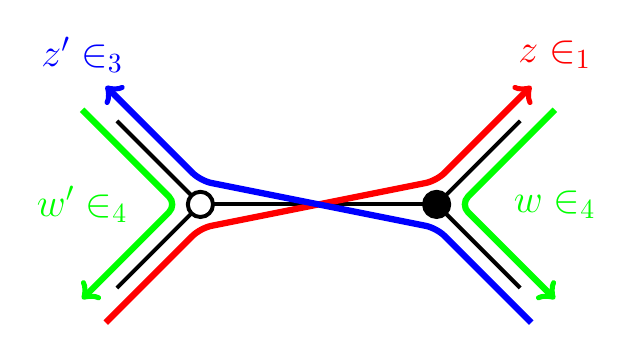
\begin{tikzpicture}
\newcommand{\edgewidth}{0.05cm}
\newcommand{\nodewidth}{0.05cm}
\newcommand{\noderad}{0.16}

\coordinate (W1) at (0,0); \coordinate (B1) at (3,0);
\path (W1) ++(135:1.5cm) coordinate (W1a); \path (W1) ++(225:1.5cm) coordinate (W1b);
\path (B1) ++(45:1.5cm) coordinate (B1a); \path (B1) ++(315:1.5cm) coordinate (B1b);

\draw [line width=\edgewidth] (W1)--(B1); \draw [line width=\edgewidth] (W1)--(W1a); \draw [line width=\edgewidth] (W1)--(W1b);
\draw [line width=\edgewidth] (B1)--(B1a); \draw [line width=\edgewidth] (B1)--(B1b);
\draw [line width=\nodewidth, fill=white] (W1) circle [radius=\noderad] ;
\draw [line width=\nodewidth, fill=black] (B1) circle [radius=\noderad] ;

\path (W1) ++(270:0.3cm) coordinate (W1-); \path (W1) ++(90:0.3cm) coordinate (W1+);
\path (B1) ++(270:0.3cm) coordinate (B1-); \path (B1) ++(90:0.3cm) coordinate (B1+);
\path (W1-) ++(225:1.7cm) coordinate (W1--); \path (W1+) ++(135:1.7cm) coordinate (W1++);
\path (B1-) ++(315:1.7cm) coordinate (B1--); \path (B1+) ++(45:1.7cm) coordinate (B1++);
\draw [->, rounded corners, line width=0.08cm, red] (W1--)--(W1-)--(B1+)--(B1++) ;
\draw [->, rounded corners, line width=0.08cm, blue] (B1--)--(B1-)--(W1+)--(W1++) ;

\path (W1) ++(180:0.3cm) coordinate (W1w); \path (W1w) ++(135:1.7cm) coordinate (W1w+); \path (W1w) ++(225:1.7cm) coordinate (W1w-);
\path (B1) ++(0:0.3cm) coordinate (B1e); \path (B1e) ++(45:1.7cm) coordinate (B1e+); \path (B1e) ++(315:1.7cm) coordinate (B1e-);
\draw [->, rounded corners, line width=0.08cm, green] (W1w+)--(W1w)--(W1w-) ;
\draw [->, rounded corners, line width=0.08cm, green] (B1e+)--(B1e)--(B1e-) ;
\node[red] at (4.5,1.9) {\Large $z\in\calZ_1$}; \node[blue] at (-1.5,1.9) {\Large $z^\prime\in\calZ_3$};
\node[green] at (-1.5,0) {\Large $w^{\prime}\in\calZ_4$} ;
\node[green] at (4.5,0) {\Large $w\in\calZ_4$} ;
\end{tikzpicture} } }
\end{center}
\caption{Zigzag paths around the intersection~$E$}\label{behavior_zigzag}
\end{minipage}

\begin{minipage}{0.49\hsize}
\begin{center}
{\scalebox{0.7}{
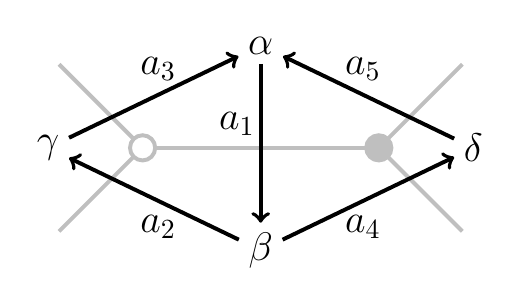
\begin{tikzpicture}
\newcommand{\edgewidth}{0.05cm}
\newcommand{\nodewidth}{0.05cm}
\newcommand{\noderad}{0.16}

\coordinate (W1) at (0,0); \coordinate (B1) at (3,0);
\path (W1) ++(135:1.5cm) coordinate (W1a); \path (W1) ++(225:1.5cm) coordinate (W1b);
\path (B1) ++(45:1.5cm) coordinate (B1a); \path (B1) ++(315:1.5cm) coordinate (B1b);

\draw [lightgray, line width=\edgewidth] (W1)--(B1); \draw [lightgray, line width=\edgewidth] (W1)--(W1a); \draw [lightgray, line width=\edgewidth] (W1)--(W1b);
\draw [lightgray, line width=\edgewidth] (B1)--(B1a); \draw [lightgray, line width=\edgewidth] (B1)--(B1b);
\draw [lightgray, line width=\nodewidth, fill=white] (W1) circle [radius=\noderad] ;
\draw [lightgray, line width=\nodewidth, fill=lightgray,] (B1) circle [radius=\noderad] ;

\node (Va) at (1.5,1.3) {\Large $\alpha$}; \node (Vb) at (1.5,-1.3) {\Large $\beta$};
\node (Vc) at (-1.2,0) {\Large $\gamma$}; \node (Vd) at (4.2,0) {\Large $\delta$};
\draw [->, line width=\edgewidth] (Va)--(Vb); \draw [->, line width=\edgewidth] (Vb)--(Vc); \draw [->, line width=\edgewidth] (Vc)--(Va);
\draw [->, line width=\edgewidth] (Vb)--(Vd); \draw [->, line width=\edgewidth] (Vd)--(Va);
\node at (1.2,0.3) {\Large $a_1$}; \node at (0.2,-1) {\Large $a_2$}; \node at (0.2,1) {\Large $a_3$};
\node at (2.8,-1) {\Large $a_4$}; \node at (2.8,1) {\Large $a_5$};
\end{tikzpicture} } }
\end{center}
\caption{The arrows around $w_E$ and $b_E$}\label{behavior_PM}
\end{minipage}
\end{tabular}
\end{figure}

Let $(Q,W_Q)$ be the QP associated with $\Gamma$. Thus, $\calP\coloneqq\calP(Q,W_Q)$ is a semi-steady NCCR of $R$ that is not steady. Let $\alpha,\beta,\gamma,\delta$ be vertices of $Q$ appearing around $w_E,b_E$ and $a_1,\dots,a_5$ be arrows between these vertices as shown in Figure~\ref{behavior_PM}. Thus, these arrows give divisorial ideals $T_{a_1}=T(1,1,0,0)$, $T_{a_3}=T_{a_4}=T(0,0,1,0)$, and $T_{a_2}=T_{a_5}=T(0,0,0,1)$. Thus, we see that
\[
\begin{aligned}
e_\alpha\calP&\cong (e_\beta\calP\otimes_RT_{a_1})^{**},&&& e_\gamma\calP&\cong (e_\alpha\calP\otimes_RT_{a_3})^{**}\\
e_\delta\calP&\cong (e_\alpha\calP\otimes_RT_{a_5})^{**},&&& e_\beta\calP&\cong (e_\gamma\calP\otimes_RT_{a_2})^{**}\cong(e_\delta\calP\otimes_RT_{a_4})^{**}.
\end{aligned}
\]

Let $v_1^\prime,\dots,v_4^\prime\in\ZZ^2$ be the vertices of the toric diagram of $R$ corresponding to $\sfP_1,\dots,\sfP_4$ respectively. Let $v_i\coloneqq(v_i^\prime,1)$ for $i=1,\dots,4$. Then, the cone $\sigma$ generated by $v_1,\dots,v_4$ defines $R$. Let $D_i\coloneqq[T(\delta_{i1},\dots,\delta_{i4})]\in\Cl(R)$ for $i=1,\dots,4$, where $\delta_{ij}$ is the Kronecker delta. Thus, we have $[T_{a_1}]=D_1+D_2,\, [T_{a_3}]=[T_{a_4}]=D_3,\, [T_{a_2}]=[T_{a_5}]=D_4$. By Lemma~\ref{cl_toric}, these satisfy
\begin{equation}\label{relations_divisor}
v_1D_1+v_2D_2+v_3D_3+v_4D_4=0.
\end{equation}

By Lemma~\ref{lem_semi}, there is a splitting generator $M=\bigoplus_{i\in Q_0}M_i$ such that $\calP\cong\End_R(M)$ and $e_i\calP\cong M$ or $M^*$ for any $i\in Q_0$. Let $\calM\coloneqq\{[M_i]\in\Cl(R)\mid i\in Q_0\}$. If $(M\otimes_RI)^{**}\cong M$ holds for a divisorial ideal $I$, then we have $[I]\in\calM$ because $M$ is a generator. Using the above isomorphism again, we have $2[I]\in\calM$. Repeating this argument, we see that $[I]$ is a torsion element in $\Cl(R)$ because of the finiteness of $\calM$. Here, we assume that $D_4$ is torsion in $\Cl(R)$, and hence there is a positive integer $a$ such that $aD_4=0$ in $\Cl(R)$. By Lemma~\ref{cl_toric}, the equation $aD_4=0$ can be obtained by the relation~\eqref{relations_divisor}. Thus, for the $3\times 3$ matrix $V\coloneqq(v_1\,v_2\,v_3)$, there exists a unimodular matrix $U$ such that one of rows of $UV$ is the zero vector. This means that $sa_1+tb_1=sa_2+tb_2=sa_3+tb_3$ for some $(0,0){\neq}(s,t)\in\ZZ^2$ where $v_i={}^t(a_i,b_i,1)$. We easily see that it is impossible to take such $(s,t)$ because the lattice points $v_1^\prime,v_2^\prime,v_3^\prime$ do not lie on the same line in $\RR^2$. Thus, $D_4$ is not torsion in $\Cl(R)$. By a similar argument, we also see that $D_3$ is not torsion. By these observations, we have
\[
e_\alpha\calP\not\cong e_\gamma\calP,\quad e_\alpha\calP\not\cong e_\delta\calP,\quad e_\beta\calP\not\cong e_\gamma\calP,\quad e_\beta\calP\not\cong e_\delta\calP.
\]
If $e_\alpha\calP\cong M$, then we have that $e_\beta\calP\cong M, e_\gamma\calP\cong M^*$ and $e_\delta\calP\cong M^*$, and hence
\begin{align}\label{eq_proof1}
M^*&\cong e_\gamma\calP\cong(e_\alpha\calP\otimes_RT_{a_3})^{**}\cong(M\otimes_RT_{a_3}),
\\
\label{eq_proof2}
M&\cong e_\beta\calP\cong(e_\delta\calP\otimes_RT_{a_4})^{**}\cong(M^*\otimes_RT_{a_4}).
\end{align}
Let $\calM^*\coloneqq\{[M_i^*]=-[M_i]\in\Cl(R)\mid i\in Q_0\}$. Then, by~\eqref{eq_proof1} we have $D_3\in\calM^*$. Using~\eqref{eq_proof2}, we then have $2D_3\in\calM$. Since $D_3$ is not torsion, we can repeat these arguments infinitely, but this contradicts the finiteness of $\calM$. Even if $e_\alpha\calP\cong M^*$, we have the same conclusion by a similar argument. Therefore, the toric diagram of $R$ is a parallelogram.
\end{proof}
